\documentclass[a4paper, article, english, oneside, unknownkeysallowed, 12pt]{memoir} 
\usepackage{preamble}


\usepackage[
backend=biber,
style=authoryear-ibid,
maxcitenames=2, % show up to 2 authors in citations
mincitenames=1, % use "et al." if more than 2
maxbibnames=10, % show up to 10 names in bibliography
minbibnames=1,
uniquelist=false,
uniquename=false
]{biblatex}


\addbibresource{causal_effect_schools.bib}

\AtEveryBibitem{%
  \clearfield{urlyear}%
  \clearfield{urlmonth}%
  \clearfield{urlday}%
  \clearfield{urldate}%
}

% Name and Title
\title{Do High Schools Shape College Choices? Evidence from Centralized Assignment in Chile}
\author{ Bruno E. Aravena-Magüida}
\date{September 2026}

% Header (top) and footer (bottom)
\pagestyle{fancy}
\fancyhead[R]{\emph{Do High Schools Shape College Choices?}}
 \fancyhead[L]{BEAM} % keep section names
\fancyfoot[R]{}
\fancyfoot[L]{}


\begin{document}

% Prints title block from macros given above
\maketitle

\begin{abstract}
School quality is usually measured with test scores, but high schools may also shape students' college choices.
This paper studies this question in Chile, where centralized assignment creates lottery variation in high-school offers.
I link assignment records to administrative data on school enrollment, standardized achievement, and higher-education applications and enrollment.
I estimate observational school value added for math, verbal achievement, enrollment in high-premium institutions and high-premium fields, and projected program income, using a rich set of pre-treatment controls.
I then test whether lottery-induced attendance at higher-value-added schools improves the corresponding outcome, controlling for expected value added in each student's assignment portfolio.
% [FIX] Abstract numbers are the July estimates. Sept main table: math 1.197, verbal 1.031, HP-inst 0.667, HP-field 0.861, log income 1.060 (+ exam-taking 0.486, benefits 0.584). Heterogeneity and horse-race sentences below refer to sections now commented out.
Achievement forecast coefficient estimates are 0.884 for math and 0.885 for verbal achievement, close to benchmarks from settings with lagged test scores.
Higher-education value added also predicts causal changes in later choices: pass-through is 0.497 for high-premium-institution enrollment, 0.803 for high-premium-field enrollment, and 0.311 for log projected program income.
Heterogeneity estimates suggest that the pass-through of math value added varies across the baseline math achievement distribution.
Gender also reveals important heterogeneity in achievement pass-through, with value added more informative for girls.
Lastly, an ordered value-added horse race shows that projected-income gains are not primarily summarized by math value added, but rather by other dimensions of value added.
High schools therefore shape college choices through dimensions of school value that achievement value added alone does not capture.
Choices that appear to reveal student preferences may thus partly reflect the information, expectations, and preparation produced by the high school attended.
\end{abstract}

% Prints a table of contents
\setcounter{tocdepth}{2}
\renewcommand\contentsname{}
%\tableofcontents* 

\clearpage
\section{Introduction}

School quality is usually summarized by achievement.
This is natural: test scores are widely available, comparable across schools, and even predictive of later outcomes \parencite{chetty_how_2011}.
But school and teacher effects are not necessarily one-dimensional.
Recent work shows that schools and teachers can affect attendance, behavior, crime, teenage motherhood, labor-market outcomes, and other long-run outcomes in ways that are only weakly related to test-score effects \parencite{jackson_what_2018, beuermann_what_2023, rose_effects_2022, angrist_methods_2023}.
Families and policymakers might therefore care about school quality measures that capture more than just achievement.

This broader view of school quality is especially relevant for high schools.
High schools are the last formal educational institutions students attend before making higher-education choices, and those choices are immensely consequential.
Whether students enter higher education, which institutions they attend, and which fields they choose all matter because returns vary substantially across institutions and, especially, fields of study \parencite{kirkeboen_field_2016}.
Yet many measures of school effects on higher education are coarse, focusing on indicators for enrollment or persistence rather than on the type of institution or field students enter.

There are also good reasons to think that higher-education choices are shaped by frictions that schools may influence.
Prior work documents large differences in application and enrollment behavior across groups of students, and shows that relatively small interventions can change college search, application behavior, and major choice \parencite{hoxby_what_2015, dynarski_closing_2021, hastings_informed_2016, chetty_diversifying_2025}.
If high schools differ in counseling, information provision, expectations, peer norms, academic confidence, or preparation for particular fields, then their effects on higher education may extend beyond their effects on achievement.

This possibility also changes how higher-education choices should be interpreted.
Decisions not to continue to higher education, to avoid particular fields, or to attend lower-quality institutions are often viewed as revealing stable preferences or privately optimal responses to expected returns.
Yet expected returns and the options students perceive may themselves depend on the information, preparation, and support provided by their high school.
A choice can therefore be privately optimal given beliefs and preparation that the school helped produce, while still being causally affected by the school attended.
This distinction is especially relevant in settings where families have limited information about educational options and access to counseling varies across schools.

This paper asks whether high schools causally affect higher-education choices, and whether those effects are captured by traditional achievement value added.
The main empirical challenge arises from the fact that students and families sort across schools.
Families choose schools based on resources, preferences, networks, location, and expectations; these same characteristics may also shape later higher-education choices.
As a result, differences across schools may reflect both causal school effects and the underlying characteristics of the students and families who select into them.

I address this challenge using Chile's centralized school assignment system, the Sistema de Admisi\'on Escolar (SAE).
SAE assigns students to public and private-subsidized schools through a centralized mechanism that uses random tie-breakers when schools are oversubscribed.
The system covers a large national school sector, allowing me to study school effects at a scale that is unusual in lottery-based designs.
This assignment variation can be linked to administrative data covering school enrollment, standardized tests, and higher-education applications and enrollment.
Linking random assignment in the mechanism to higher-education choices allows me to answer this question in a national context.


The analysis proceeds in two steps.
First, I estimate observational value added for each school and outcome in the broad panel.
These measures are school fixed effects from regressions that adjust for rich pre-treatment controls, including grade-4 standardized test scores, family-background variables, and middle-school controls.
Second, I validate these value-added measures for each school using the SAE lottery offers as exogenous variation.
% [UNCLEAR] 'together with the value added measured in the first step' is unclear: say that the instrument is offered-school VA and the treatment is attended-school VA.
I instrument for attended school with the school offered through the centralized mechanism, while controlling for the expected value added that arises from the probabilities of assignment of the student to the schools in their list, together with the value added measured in the first step.


I summarize this relationship with a forecast coefficient, $\psi$, in line with \textcite{angrist_leveraging_2017}\footnote{I refer to the forecast coefficient as pass-through interchangeably}.
If $\psi=1$, then the causal effect induced by complying with a lottery offer equals the gain predicted by observational value added for that outcome.
If $\psi=0$, the observational value-added measure has no causal predictive content along the lottery-induced margin.
The main estimates suggest meaningful pass-through.
% [FIX] July numbers; update to Sept table. 'causal effects are smaller than the value-added might suggest' no longer holds for math (1.197) and income (1.060).
For achievement, the estimates are 0.884 for math and 0.885 for verbal achievement.
For higher-education choices, the forecast coefficients are 0.497 for enrollment in a high-premium institution, 0.803 for enrollment in a high-premium field, and 0.311 for log projected program income.
In practical terms, schools that observationally look better at raising achievement or higher-education outcomes also predict causal effects on those same outcomes, though the causal effects are smaller than the value-added might suggest.
%The achievement estimates are close to comparable validation estimates in \textcite{angrist_leveraging_2017} despite the absence of immediately lagged outcomes.
%This validates the rich set of pre-treatment controls used here, which can also be applied to outcomes, such as higher-education choices, for which lagged measures are unavailable.

%I then ask for whom observational value-added measures are most informative.
%%Splitting the sample by baseline grade-4 math achievement shows that, relative to students in the middle quintile, math value added is substantially less predictive in the bottom quintile and marginally more predictive in the top quintile.
%Math and verbal achievement also show statistically significant differences by gender: achievement value-added measures are less informative for boys.
%These results point to meaningful heterogeneity in achievement, yet remarkable stability for the other higher-education dimensions.

%Finally, I examine which dimensions of school value added best predict gains in projected program income, a proxy for later earnings.
%For interpretation, I use an ordered horse race: math value added enters first, high-premium-institution value added enters after removing its school-level association with math, and high-premium-field value added enters after removing its association with the first two dimensions.
%In this specification, the incremental high-premium-field dimension remains positive and precisely estimated, while math value added does not carry the projected-income signal once the higher-education choice dimensions are included.
%These results are difficult to reconcile with a view in which math achievement fully summarizes the school dimensions relevant for projected income.

The paper contributes to three literatures.
First, it contributes to work on teacher and school value added.
A large literature estimates the effects of teachers and schools on test scores and longer-run outcomes \parencite{chetty_measuring_2014, dobbie_medium-term_2015, jackson_what_2018, beuermann_what_2023, rose_effects_2022}.
This work increasingly emphasizes that test-score value added may miss important dimensions of educational production.
I extend this idea to high-school effects on higher-education choices, focusing not only on enrollment or achievement but also on whether students enter high-premium fields, high-premium institutions, and programs with higher projected earnings.


Second, the paper contributes to the literature using lotteries and centralized assignment systems to estimate school effects \parencite{abdulkadiroglu_elite_2014, abdulkadiroglu_research_2017, angrist_credible_2024}.
In the spirit of \textcite{angrist_leveraging_2017}, I ask whether observational value-added measures are useful guides to causal school effects.
The contribution here is to apply this pass-through logic to a national high-school assignment system and to outcomes observed after students transition into higher education.

Third, the paper contributes to work on higher-education choice.
Prior research shows that the field and institution students choose matter for later outcomes, and that information and application frictions can change those choices \parencite{kirkeboen_field_2016, hoxby_what_2015, dynarski_closing_2021, hastings_informed_2016, chetty_diversifying_2025}.
I study high schools as a possible upstream source of these differences.
Rather than evaluating a particular counseling or information intervention, the paper measures whether the high-school system itself generates causal differences in students' higher-education paths.

The rest of the paper is organized as follows.
Section 2 describes the Chilean setting and the linked administrative data.
Section 3 presents the empirical framework.
% [FIX] Roadmap outdated: new Sec. 4 (applications/compliers), results are now Sec. 5, heterogeneity and horse race are commented out, var/cov section is new. Use \ref.
Section 4 reports the main results, heterogeneity by baseline achievement and gender, and the ordered value-added horse race for projected program income.
Section 5 concludes.

\clearpage
\section{Context and Data}

\subsection{Institutional Setting}

Chile is a useful setting for this project because national administrative data records school enrollment, academic histories, standardized achievement, and higher-education choices with individual identifiers that allow students to be matched across educational data.

Formal secondary education begins in grade 9 and lasts four years.
Students may attend public, private-subsidized, or private non-subsidized schools.
Public and private-subsidized schools are fully or partly financed by the State and thus participate in the centralized school assignment system described below.
They serve 90.6\% of the high-school population. Private non-subsidized schools remain outside that mechanism and serve the remaining 9.4\%.

%In the broad grade-8 universe used in the value-added analysis, private non-subsidized schools account for about 9.4\% of students.
%The lottery-based sample is therefore given by the set of students who apply for for entrance to grade 9 in a school in the public and private-subsidized sector after 


\subsection{Centralized School Assignment}

Chile's centralized school assignment system, the Sistema de Admisi\'on Escolar (SAE), assigns students to participating schools through a version of student-proposing Deferred Acceptance.
Families submit ranked lists of schools.
The mechanism combines these rankings with school vacancies and priority rules, and it uses random tie-breakers when there are more applicants than seats within a priority group.
If a student's offered school depends on one of these tie-breakers in the system, different lottery draws will imply different school assignments.
% [UNCLEAR] Awkward; also the draft switches between 'I' and 'we'/'us'/'our' (here, 'allowing us', 'we can track', 'we can see', 'our rich set'). Pick one.
We say therefore this student is at assignment risk.  Conditional on the information that determines priorities and assignment probabilities, these tie-breakers or lotteries generate the quasi-experimental variation in school assignment for students with assignment risk as described by \textcite{abdulkadiroglu_research_2017}.


SAE started in 2017 in some regions and was rolled out nationally in 2018. 
% [FIX] Lottery sample is now 2018--2020 cohorts (Table 1, Sec. 2.3.2). Also check graduation years: with grade-8 cohorts 2018--2020, expected graduation is 2022--2024, not 2023--2025 (cf. the cohort-2019 example below: graduate 2023).
Given that I study high school effects, I use applications to grade-9 vacancies between 2018 and 2021. 
These cohorts are expected to finish high school between 2023 and 2025, allowing us to observe high school attendance and post-schooling outcomes.

Implementing this design requires recovering each applicant's probability of assignment to each school among those in the submitted rankings of schools.
I do this by replicating the SAE assignment algorithm and repeatedly simulating counterfactual lottery draws, which determines which students are at assignment risk.
As a diagnostic check, when I run the replicated algorithm using the original lottery numbers for the 2018--2020 regular grade-9 processes, I reproduce over 99\% of observed first-round assignments in each of the three cohorts. \footnote{Even though SAE runs two additional rounds, these complementary rounds are very limited in sample size. Since they assign vacancies in previously undersubscribed schools, assignment risk is unlikely in these rounds.}
The remaining mismatch reflects institutional features that are difficult to fully recover from public documentation, but the high replication rate gives confidence that the simulated probabilities capture the relevant assignment risk.


This centralized system is very relevant to determine the high school attended.
Figure \ref{fig:first-stage} makes this point by showing attendance rates in the 100 most demanded schools, with different markers for applicants with and without first round offers.


\begin{figure}[!htbp]
\centering
\includegraphics[width=\textwidth]{../../output/figures/compliance/school_level_offer_attendance_first_stage_top100.png}
\caption{Effect of SAE offers on attendance}
\label{fig:first-stage}
\end{figure}


For this exercise and the rest of the paper, I define high-school attendance as the school where a student spends the most time after grade 8, with most recent spells breaking ties.
This definition smooths over short enrollment spells and transfers, and it assigns a single high-school value to each student.
As a result, students who did not receive a first-round offer might still end up attending a certain high-school via complementary rounds or an application cycle in a later year.
On average, a high school is attended at a rate of 6.9\% by the first-round rejected students and at a rate of 62.5\% by the accepted students. 
% [FIX] 62.5 - 6.9 = 55.6; rounding or a typo?
This suggests an average effect of the first-round offer of 55.5 percentage points, making it a relevant instrument for school attendance.



%The estimation sample consists of timely SAE applicants: students who apply in the assignment process corresponding to their grade-8 cohort and who have assignment risk in the simulated data.
%Assignment risk means that the simulated assignment probabilities do not place all probability mass on a single school.


%As shown in Table~\ref{tab:data-samples}, 135,916 students across the 2018--2020 cohorts have a valid high-school exposure, are ages 12--16, have complete lottery controls, apply to SAE on time, and face assignment risk.
%The score-based estimation sample further restricts to the 108,418 lottery-risk students with an observed math or verbal national admission-test score.
%On average, these students have positive simulated assignment probability at about 3.1 schools; the median is 3 and the 90th percentile is 5.

%Among applicants with assignment risk, 85.4\% receive a first-round SAE offer.
%The remaining 14.6\% have no first-round assignment (\texttt{rbd\_admitido}) in the regular-process results; they are retained, with their first-round offer value set to zero.
%The first-round offered RBD is the source of lottery variation, while the student's realized high-school exposure is measured by the most-time RBD described above.

%The value-added exercise uses the broader complete-control panel, while the causal estimates use the smaller lottery-risk sample.
%This distinction is central to the interpretation.
%The broad panel improves precision in estimating school-level outcome gradients, and the lottery sample then tests whether those observational value-added measures have causal signal on the centralized-assignment margin.
%The results therefore speak most directly to students and schools represented in the SAE lottery-risk sample.
%Because SAE covers the public and private-subsidized sector, this is a large and policy-relevant part of the high-school market, but extrapolating to private non-subsidized schools or non-lottery margins requires assuming that the same value-added gradients are comparable there.


\subsection{Sample Description}

In this subsection I describe the samples I employ for the two steps of my analysis. 
% [FIX] VA is defined as school fixed effects (eq. 2), not residuals. 'as representative as possible' is also vague.
In my first step, I construct measures of value added of schools in different outcomes as residuals in a regression with rich covariates and as representative as possible.
I refer to the sample used for that exercise as the value added sample.
In the second step, I use the exogenous variation in the centralized mechanism to study whether school changes due to tie-breakers are as predictive of effects as the value added metric suggest. 
For that exercise I collect all students with assignment risk in their grade-9 SAE application.
I refer to this sample as the lottery sample. 


\subsubsection{Value Added Sample}

I construct the value added sample by merging annual enrollment, grade progression, attendance, grades, and completion records using the student identifier provided for educational data.
The linked administrative panel starts from the universe of students first observed in grade 8 between 2017 and 2020, producing 944,510 students across four cohorts, defined 
by their year of grade-8 enrollment. 
For instance, a student in the 2019 cohort who wants to change schools within the non-private system applies to SAE that year, is expected to start high school in 2020, and is expected to graduate in 2023.

%If a student in cohort 2019 intends to attend high school in a non private institution 
% is expected to apply that year to the centralized assignment mechanism for entrance to grade 9 in 2020 and has expected graduation in 2023.

To construct value-added for each school I keep as much from this broad panel as possible, while ensuring the comparison is reasonable.
From this universe I drop students younger than 12 or older than 16 in grade 8 and those who do not attend high school. 


% [UNCLEAR] 'this' is ambiguous: say explicitly that requiring a complete control vector is the most binding restriction.
Given that value-added estimation relies on a rich set of baseline covariates, this becomes the most important restriction on this sample.
For these covariates, I use information from Chile's national standardized assessment system (SIMCE) and middle school relative performance.
Middle school controls are constructed by comparing attendance and GPA of a student to those of their peers in middle school every year. 
These are then averaged and summarized into two middle school z-scores for a student: one for attendance and one for GPA.

SIMCE exams are administered in different grades depending on the year. 
This always includes grade 4 and occasionally grades 8 and/or 10.
Unfortunately grade-8 and grade-10 measures are not available for all the studied cohorts.
I therefore use grade-4 SIMCE as the main pre-treatment achievement control.

SIMCE also collects parent surveys.
I use these surveys to measure family background before treatment, including household income, parental education, indigenous origin of the parents, and early-childhood education.
These variables are useful because they proxy for family resources and prior investments that may influence both high-school choices and later higher-education outcomes.
When parent-survey variables are missing, I use middle school and neighborhood cells to impute medians where enough donor observations are available; remaining missing values are left missing.


%I define a middle school --with a similar role  for those students that can be tracked in the anual enrollment database, 
As can be seen in Panel A of Table \ref{tab:data-samples}, from the original 944,510 students in these cohorts, 
I keep the 757,999 for which I have a complete control vector with all the sources of information described above. 
Sample restrictions defined in each row should be read cumulatively within each panel.



\begin{table}[H]
\centering
\caption{Construction of the value-added and SAE samples}
\label{tab:data-samples}
\begin{minipage}[t]{0.48\textwidth}
\centering
\textbf{Panel A: Value-added sample}\\[0.4em]
\begin{tabular}{@{}p{0.72\linewidth}r@{}}
\toprule
Sample restriction & Students \\
\midrule
Cohorts 2017--2020 & 944,510 \\
+ valid HS and age 12--16 & 931,547 \\
+ complete VA control set & \textbf{757,999} \\
+ admission test & 622,809 \\
\bottomrule
\end{tabular}
\end{minipage}
\hfill
\begin{minipage}[t]{0.48\textwidth}
\centering
\textbf{Panel B: SAE lottery sample}\\[0.4em]
\begin{tabular}{@{}p{0.72\linewidth}r@{}}
\toprule
Sample restriction & Students \\
\midrule
Cohorts 2018--2020 & 706,042 \\
+ valid HS and age 12--16 & 696,817 \\
+ complete lottery control set & 587,142 \\
+ application in SAE & 241,490 \\
+ assignment risk & \textbf{135,916} \\
+ admission test & 108,418 \\
\bottomrule
\end{tabular}
\end{minipage}
\end{table}



\subsubsection{Lottery Sample}


For the lottery sample I start following virtually the same steps but with the 2018--2020 cohorts, the first ones with SAE rolled out at a national level.
Panel B of Table \ref{tab:data-samples} repeats the accounting exercise above for the lottery sample. 
% [FIX] Text 706,402 vs table 706,042; text 241,190 (next line) vs table 241,490.
From an original list of 706,402 we can track the baseline set of controls for only 587,142. 
Out of that group only about 41\% (241,190) applied for a change of school through the SAE mechanism for a spot in grade 9\footnote{I consider only applications to grade 9 in the year the student is in grade 8, to avoid including students who changed schools after failing a grade}.
In some cases, students (e.g., those applying to undersubscribed schools) are guaranteed an offer to a certain school. 
The assignment mechanism does not yield exogenous variation for such cases since there is no tie-breaking.
As a result, the SAE lottery sample (135,916) only considers those students whose preferences imply non-trivial assignment probabilities. 



%For the value-added sample, I then retain the 2017--2020 cohorts, leaving 944,510 students across four cohorts.
%I make this cohort restriction because these cohorts have comparable grade-4 SIMCE baseline controls; the 2021 cohort does not.
%The main high-school exposure is observed for 4,133 schools with a unique identifier (RBD).
%I define high-school exposure as the school identifier where a student spends the most time after grade 8.
%I define middle-school attendance analogously as the RBD where the student spends the most time in grades 5 to 8.
%The same histories let me construct pre-treatment middle-school controls, including standardized measures of grades and attendance before high school.


%Table~\ref{tab:data-samples} summarizes how the linked administrative sources map into the two samples used in the analysis.
% [FIX] The validation sample is the at-risk sample (135,916), not only exam-takers, and the design validates all outcomes, not only score-based ones. The next sentence ('which is when the last row becomes relevant') is unclear.
The broad complete-control panel is used to estimate the main school value-added measures, while the SAE lottery exam-taker sample is used to validate score-based value-added measures using assignment variation.
For some outcomes, I condition the samples to test-takers which is when the last row becomes relevant.

\subsection{Characterization of the samples}

\textit{How different are these two samples?} Table \ref{tab:balance_samples} helps us answer this question. 
% [FIX] Column numbers skip column (2)/(3) in this sentence vs. the next paragraphs; check against the table layout.
Here, I report means on some key variables for the broad panel (column 1), 
students that applied for a HS in SAE (column 2) and their subset which had applications with assignment risk (column 4).

\input{../../output/tables/balance_table/balance_table_samples.tex}


Column (3) report differences between SAE applicants and the broad sample. 
From there we can see that the sample of students that apply for a new school in grade 9 are negatively selected relative to the population:
For instance, they perform around 0.2 SD below in achievement tests in grade 4, on average have mothers with one fewer year of education and perform 0.3 SD worse in exams to higher education.
The joint test clearly rejects that the two populations are similar.

% [UNCLEAR] Say which groups column (5) compares (at-risk vs. broad panel?). Otherwise the reader has to reconstruct it from the table.
Column (5) shows a comparable pattern, but with smaller differences.
Column (6) makes it clear that students with assignment risk are positively selected relative to those without, 
with the respective joint test also rejecting that the two groups are similar. 

The differences present in (5) could make one worry that estimates run on the broad panel might not be useful to predict effects on the population of SAE applicants with assignment risk.
For this to be an issue, SAE applicants at-risk would need to be different from those of the broad sample in ways that our rich set of controls does not capture. 
If that were the case, the validation step of the design would show that the VA estimated are biased and not as predictive of causal effects.
At its core, the validation step answers whether estimates in sample (1) predict causal effects in sample (4).


\subsection{Higher Education Outcomes}

The higher-education system also generates administrative data on applications, admission scores, and enrollment.
Taking the national admission exam is a choice for secondary-school students, but it is the standard route into selective higher education.
Students who apply through the centralized admission system take mandatory math and verbal components, and may also take optional subject exams.\footnote{The national admission exam was called the PSU through 2020, the PTU in 2021--2022, and the PAES from 2023 onward.}
I use the mandatory math and verbal scores as achievement outcomes, standardizing them within test year to make them comparable across test regimes.

Higher-education applications and admissions are organized at the program-institution level.
A student's admission depends on entrance-exam scores, school GPA-based scores, ranked program preferences, and the weights each program assigns to score components.
This structure is useful because it makes higher-education choices much richer than a single college-enrollment indicator: students choose not only whether to enroll, but also which institution, program, and field to pursue.

Students in the sample have not yet finished higher education, so I cannot observe their realized earnings. 
I take advantage of MiFuturo, an information source run by the Ministry of Education that reports labor-market statistics at the program level.
I use its reported average income in the fourth year after graduation to assign an earnings proxy to higher-education options. 

Because the MiFuturo income file is not observed at the exact enrollment-program code used in the matricula records, I do not treat it as a direct one-to-one match for every student-program record.
Instead, I estimate log-income fixed-effect models in the MiFuturo data using institution and generic-program cells.
Figure~\ref{fig:mifuturo-field-income-premia} shows the estimated generic-program fixed effects organized by field.
I then use generic-program and institution estimates to construct projected-income measures for the matriculated programs observed in the student panel when the exact program has no direct MiFuturo value.

\begin{figure}[!htbp]
\centering
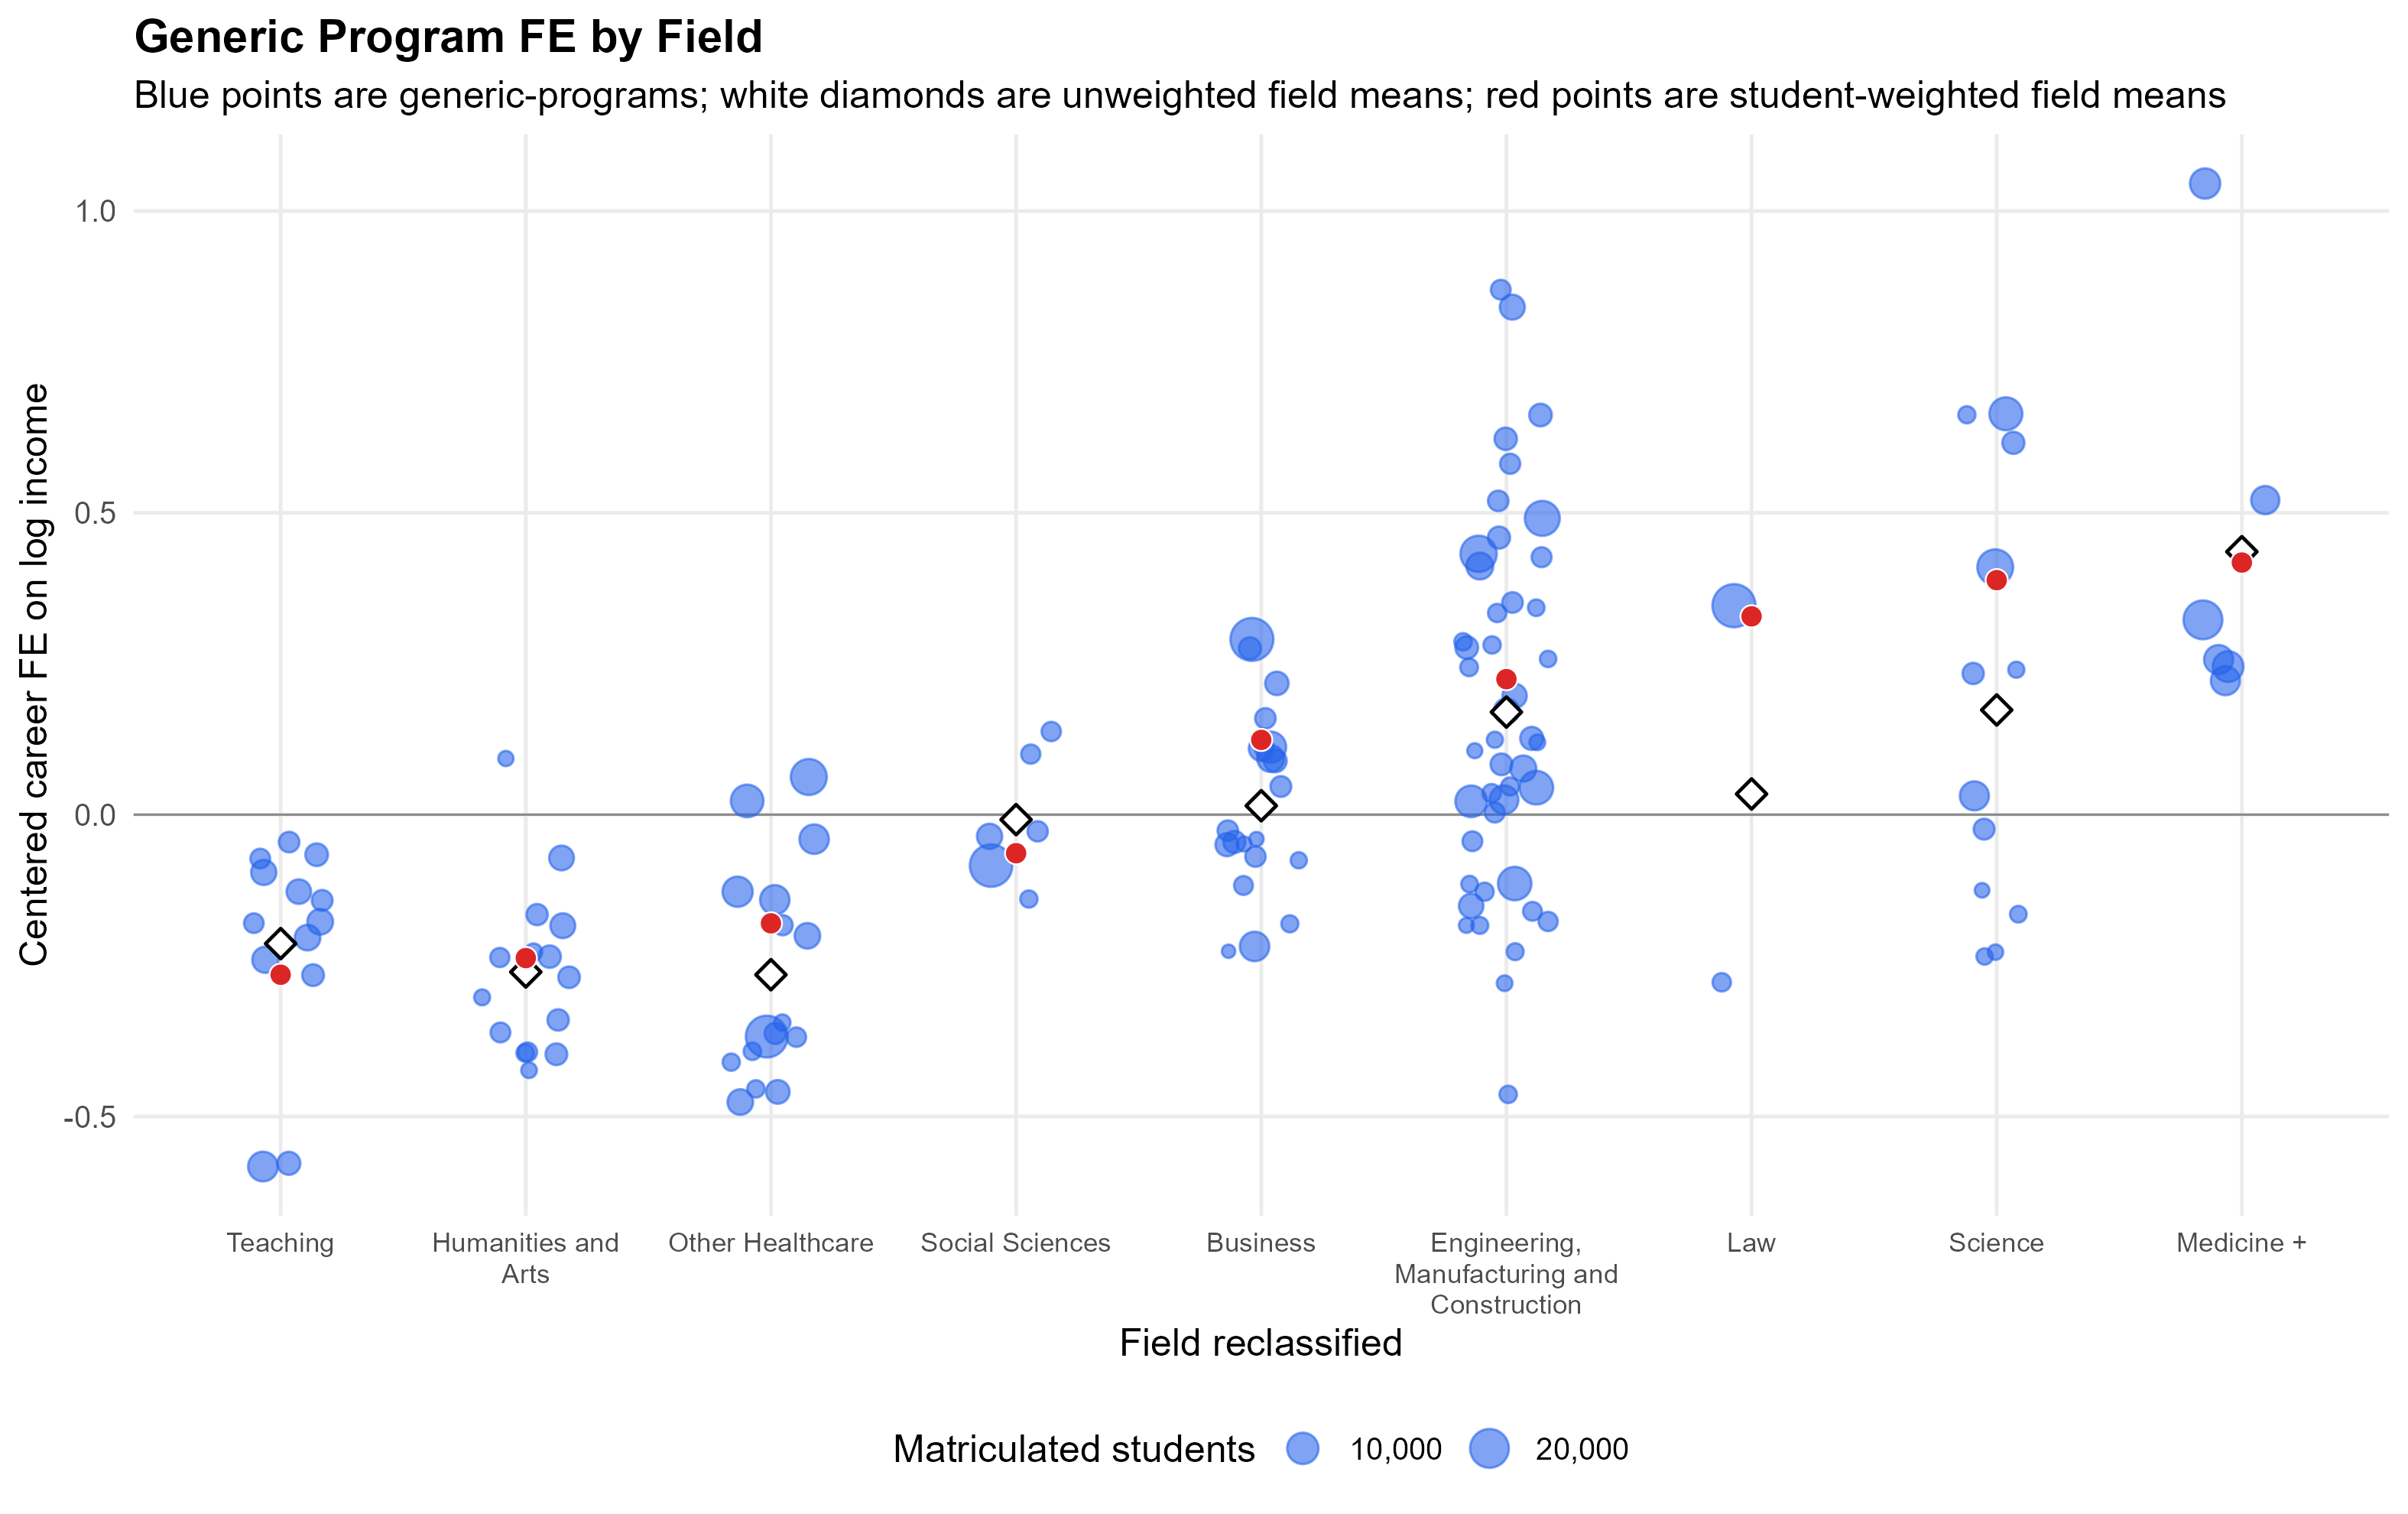
\includegraphics[width=\textwidth]{../../output/figures/mifuturo_matricula_income/area_carrera_generica_program_fe_by_field.png}
\caption{MiFuturo Generic-Program Income Premia by Field}
\label{fig:mifuturo-field-income-premia}
\end{figure}

% [FIX] 'I use three higher-education choice outcomes', but the results use seven outcomes: admission-exam taking and benefits/credit applications are never defined in the data section.
I link the school panel to higher-education enrollment records for the first observed enrollment.
I use three higher-education choice outcomes.
The first is an indicator for enrollment in a high-premium field.
This indicator equals one for students whose first observed higher-education enrollment is in Science, Law, Engineering/Manufacturing/Construction, or Medicine+\footnote{Medicine+ includes premium health-related careers such as medicine, pharmacy, nursing, midwifery, medical technology, and dentistry.
Other health and technical-health programs are not included in this high-premium-field category.}, which correspond to the right-hand side of Figure~\ref{fig:mifuturo-field-income-premia}.


The second is an indicator for enrollment in a high-premium institution.
This indicator equals one when the student's first observed matriculated institution has a particularly high institution fixed effect in the MiFuturo log-income model.\footnote{Specifically, I use a threshold of 0.1 log points relative to the average program, which roughly translates to an average institution premium of 10\%.}
Students without an observed higher-education enrollment are coded as zero for the high-premium-field and high-premium-institution indicators.

The third is log projected program income.
For matriculated students, projected program income comes from MiFuturo-based predictions using a hierarchy that first uses institution-by-generic-program fixed effects when available, then generic-program fixed effects, then institution fixed effects, and finally the global MiFuturo mean.
For students with no observed higher-education enrollment, projected program income is set to the current minimum-wage proxy of 553,553 Chilean pesos before taking logs.\footnote{This is consistent with the fact that the amounts reported in MiFuturo are in 2025 Chilean pesos.}


%For matriculated students, missing or unsupported high-premium-field classifications are left missing rather than coded as non-high-premium.
%The math and verbal score outcomes require observed national admission-test scores.
%The unconditional postsecondary outcomes instead retain students without higher-education enrollment when non-enrollment is part of the outcome definition.
%In the 2017--2020 complete-control value-added panel, 571,110 students have a math or verbal admission-test outcome.

[FIX] Talk about becas/ creditos ? 

\clearpage 
\section{Empirical Framework}

This section describes the empirical object and the research design.
The goal is not to estimate a separate causal effect for every school and every possible margin of substitution.
Instead, I ask whether an outcome-specific observational value-added measure is informative about causal effects generated by lottery-induced changes in school attendance.
The design therefore collapses school effects into scalar measures and estimates a forecast coefficient for each outcome.

\subsection{School Effects and Observational Value Added}

I use a constant-effects value-added model as a guide:
\begin{equation}
  Y_i^m(j) = \mu^m + V_j^m + \epsilon_i^m,
  \label{eq:potential-va}
\end{equation}
Here, $Y_i^m(j)$ is student $i$'s potential outcome for outcome $m$ if assigned to high school $j$.
The index $m$ denotes the outcome, and $j$ denotes the high school.
The term $\mu^m$ is the average level of outcome $m$ under the student-weighted average school.
The term $V_j^m$ is the contribution of school $j$ to outcome $m$ relative to that average.
The term $\epsilon_i^m$ captures student-level determinants of outcome $m$ that do not vary with the assigned school in this constant-effects representation.
I normalize school effects so that their student-weighted mean is zero, $\sum_j \omega_j V_j^m = 0$, where $\omega_j$ is the share of students linked to school $j$ in the value-added sample.
This centering means that the weighted average of $V_j^m$ across schools is exactly zero.
A positive $V_j^m$ therefore denotes a school above the student-weighted average for outcome $m$, while a negative value denotes a school below that average.
% [FIX] Lists five outcomes; the main table has seven.
The main outcomes are math and verbal achievement, indicators for enrollment in a high-premium field and a high-premium institution, and log projected program income. 

The first step constructs observational value added in the broad complete-control panel.
For each outcome $m$, I estimate
\begin{equation}
  Y_i^m = \alpha^m + \lambda_{s(i)}^m + X_i'\Gamma^m + u_i^m,
  \label{eq:observational-va}
\end{equation}
where $s(i)$ is the student's main high-school RBD and $X_i$ contains pre-treatment controls.
These include cohort, gender, age, a third-degree polynomial in each of grade-4 SIMCE math and language, family-background measures from SIMCE parent surveys\footnote{In particular: family income decile, years of education and indigenous status of each parent, and indicators for whether the student attended any institution before primary education.}, and middle-school controls from grades 5 to 8 (middle school indicator and school-normalized attendance and performance).
%Score outcomes are estimated among students with observed admission-test scores, while the other postsecondary outcomes use the complete-control panel after applying the outcome-specific missing-data rules described above.
I define the observational value-added measure $\widehat{V}_j^m$ as the centered empirical analogue of $V_j^m$: the estimated school fixed effect $\widehat{\lambda}_j^m$ from equation~\eqref{eq:observational-va}, centered using the same student-weighting convention.

Importantly, these fixed effects by themselves answer an observational question: conditional on $X_i$, which schools have higher average outcomes?
If school assignment in the broad panel were truly random, then the centered fixed effect $\widehat{\lambda}_j^m$ would identify $V_j^m$ up to sampling error.
In practice, students sort across schools, so the fixed effects may combine true school effects with any remaining selection not absorbed by controls.
The second step therefore asks whether the part of $\widehat{V}_j^m$ shifted by the SAE lotteries corresponds to causal effects in the same outcome.


\subsection{Assignment Risk and Expected Value Added}

SAE applicants submit rank-ordered lists of schools.
Let $Z_i$ denote the first-round school offer and $D_i$ denote the school attended, measured by the post-grade-8 most-time RBD.
A student has a preference and priority type $\theta_i$, and the assignment mechanism implies an assignment-probability vector $p_i=(p_{i1},...,p_{iJ})$, where $p_{ij}=Pr(Z_i=j)$.
Under equal treatment of equals, students with the same type have the same assignment probabilities \parencite{abdulkadiroglu_research_2017}.
For pre-treatment characteristics and potential outcomes fixed under re-randomization, we have
\begin{equation}
  (Y_i^m(1),...,Y_i^m(J), X_i) \ind Z_i \mid p_i.
  \label{eq:offer-independence}
\end{equation}

The raw vector $p_i$ is high-dimensional, because students can rank many different combinations of schools.
For an outcome-specific scalar value-added measure, I summarize assignment risk by the expected value added in the student's portfolio:
\begin{equation}
  E_i^m = \sum_j p_{ij}\widehat{V}_j^m.
  \label{eq:expected-va}
\end{equation}
This is the average value added the student would receive over repeated randomizations of the assignment mechanism, holding the submitted application and priorities fixed.
In the main IV specification, this scalar expected value replaces a large set of school-specific probability controls.

For each outcome $m$, define the value added of the attended school and offered school as
\begin{equation}
  A_i^m = \widehat{V}_{D_i}^m,
  \qquad
  O_i^m = \widehat{V}_{Z_i}^m.
  \label{eq:attended-offered-va}
\end{equation}
The instrument is $O_i^m$, the value added of the school generated by the lottery offer.
The endogenous variable is $A_i^m$, the value added of the school actually attended.
The notation is mnemonic: $O_i^m$ is the value added of the \textbf{O}ffered school, and $A_i^m$ is the value added of the \textbf{A}ttended school.
Because assignment offers vary randomly conditional on the assignment probabilities, variation in $O_i^m$ around $E_i^m$ provides quasi-experimental variation in the quality of the school offer.


\subsection{Scalar IV Specification}

The first empirical question is whether observational value added predicts causal effects on the same outcome.
Specifically, when the assignment mechanism moves a student toward a school with higher $\widehat{V}_j^m$, does outcome $m$ rise, and by how much relative to the observational difference encoded in $\widehat{V}_j^m$?
The main IV system is given by the following pair of equations:
\noindent
  \begin{equation}
    \begin{aligned}
      Y_i^m ={}& \alpha^m + \psi^m A_i^m + \rho^m E_i^m +  W_i'\delta^m + \eta_i^m,
    \end{aligned}
    \label{eq:pass-through}
  \end{equation}

  \begin{equation}
    \begin{aligned}
      A_i^m ={}& a^m + \kappa^m O_i^m + \rho_A^m E_i^m +  W_i'\delta_A^m + \nu_i^m.
    \end{aligned}
    \label{eq:first-stage}
  \end{equation}

Here, $Y_i^m$ is student $i$'s realized value of outcome $m$. The value added of the attended school, $A_i^m$, is instrumented with the value added of the school offered through the assignment mechanism, $O_i^m$.
$E_i^m$ is the expected value added implied by the student's assignment-probability vector.
Finally, $W_i$ is a parsimonious lottery-sample control vector containing cohort, gender, age, and grade-4 SIMCE math and language.
This differs from the richer control vector used to construct $\widehat{V}_j^m$ in equation~\eqref{eq:observational-va}, which also includes family-background and middle-school controls.
%The rich controls enter through the construction of the school value-added measures, while equation~\eqref{eq:pass-through} asks whether those pre-constructed measures pass through in the SAE lottery sample after conditioning on assignment risk and core baseline covariates.
All reported specifications use heteroskedasticity-robust standard errors.

The coefficient $\psi^m$ is the key object.
It measures how much of the observational value-added difference induced by the lottery offer passes through into causal effects on the same outcome.
If $\psi^m=1$, then a one-unit increase in observational value added causes a one-unit increase in the outcome.
If $\psi^m=0$, the observational measure has no causal predictive content along the lottery-induced margin.
Values between zero and one imply that observational value added is directionally informative, but overstates the causal effect of attending higher-value-added schools.

The scalar design is useful because a fully flexible school-specific IV design would be high-dimensional and would mix many margins of substitution across fallback schools \parencite{angrist_methods_2023, kirkeboen_field_2016}.
It instead asks whether movement toward schools with higher measured value added causes better outcomes, after controlling for the expected value added implied by each student's assignment risk.

% [FIX] The heterogeneity results are commented out in Sec. 5. Either restore them or drop/park this paragraph.
A second empirical question is whether the forecast differs by students' baseline achievement.
To answer that question, I also estimate equation~\eqref{eq:pass-through} separately by quintiles of baseline grade-4 math achievement or gender.
Because gender and grade-4 SIMCE are fixed before high-school assignment, these splits describe heterogeneity without conditioning on a post-treatment outcome.

\subsection{Empirical Bayes}

The school fixed effects in equation~\eqref{eq:observational-va} are estimated with different precision.
In particular, effects for schools with smaller regression samples or noisier outcomes contain more sampling error.
I therefore use an Empirical-Bayes (EB) version of the observational school-value index, which shrinks noisier estimates more strongly toward the across-school mean \parencite{walters_chapter_2024}.
For each outcome $m$, let $se_j^m$ denote the regression-derived standard error of the student-weighted centered fixed effect $\widehat{V}_j^m$.
This is the uncertainty of the same centered effect used in the scalar design, rather than the standard error of an arbitrary reference-normalized school dummy.

I estimate the latent across-school variance by subtracting average sampling variance from the student-weighted variance of the estimated effects:
\begin{equation}
  \widehat{\tau}_m^2 =
  \max\left\{
    \operatorname{Var}_{\omega}\left(\widehat{V}_j^m\right)
    - \sum_j \omega_j (se_j^m)^2,\,
    0
  \right\},
  \label{eq:eb-latent-variance}
\end{equation}
where $\omega_j$ is proportional to the number of students in school $j$'s stage-1 regression sample.
The implied school-specific reliability is
\begin{equation}
  \lambda_j^m =
  \frac{\widehat{\tau}_m^2}
  {\widehat{\tau}_m^2 + (se_j^m)^2},
  \label{eq:eb-reliability}
\end{equation}
and the EB school value is
\begin{equation}
  \widehat{V}_{j}^{m,EB}
  =
  \overline{\widehat{V}}_{\omega}^m
  +
  \lambda_j^m
  \left(
    \widehat{V}_j^m-\overline{\widehat{V}}_{\omega}^m
  \right).
  \label{eq:eb-va}
\end{equation}
Note that as $(se_j^m) \to 0$ (more precision on the estimate), $\lambda^m_j \to 1$ and the posterior approaches the original $\hat{V}_j^m$.
Otherwise, the posterior lies between the estimate $\hat{V}_j^m$ and the weighted mean of such estimates, $\overline{\widehat{V}}_{\omega}^m$.

I recenter these posterior means using the same student weights, so their student-weighted mean remains zero.

I then replace $\widehat{V}_j^m$ with $\widehat{V}_{j}^{m,EB}$ everywhere in the scalar IV construction:
\begin{equation}
  A_i^{m,EB} = \widehat{V}_{D_i}^{m,EB},
  \qquad
  O_i^{m,EB} = \widehat{V}_{Z_i}^{m,EB},
  \qquad
  E_i^{m,EB} = \sum_j p_{ij}\widehat{V}_{j}^{m,EB}.
  \label{eq:eb-iv-objects}
\end{equation}
The EB specification instruments $A_i^{m,EB}$ with $O_i^{m,EB}$ and controls for $E_i^{m,EB}$ in the same way as equation~\eqref{eq:pass-through}.
%Thus, EB improves the signal-to-noise ratio of the stage-1 observational index before it is used in the lottery design; it does not estimate a separate causal effect for each school or form a hybrid causal-EB estimator.
%Because shrinkage compresses the scale of the school-value index, the resulting forecast coefficients should be interpreted together with the distribution of the EB-shrunken index.


\subsection{Variance--Covariance Analysis}

Equation~\eqref{eq:eb-latent-variance} treats each outcome separately: it purges sampling noise from the variance of a single outcome's school-value estimates.
But the paper's motivating claim, that school effects are not necessarily one-dimensional, is fundamentally a claim about how effects on \emph{different} outcomes relate to one another across schools \parencite{jackson_what_2018, rose_effects_2022}.
Answering that question requires the covariance of the latent effects $V_j^m$ and $V_j^{m'}$ across schools, not just their individual variances.

A naive covariance of the raw estimates, $\widehat{\mathrm{Cov}}\left(\widehat V_j^m, \widehat V_j^{m'}\right)$, is not a valid estimate of $\mathrm{Cov}(V_j^m, V_j^{m'})$ for the same reason that the naive variance in equation~\eqref{eq:eb-latent-variance} required a bias correction.
Sampling error in $\widehat V_j^m$ and sampling error in $\widehat V_j^{m'}$ are both computed from the same students in the same regression sample, so they are generally correlated with each other: idiosyncratic cohort-level shocks, mechanical overlap in the estimation sample, or correlated measurement error can all generate a positive or negative covariance between the two sampling errors even if the underlying school effects $V_j^m$ and $V_j^{m'}$ are unrelated.
A plug-in covariance therefore conflates true cross-outcome covariation in school effects with correlated noise, in a way that ordinary Empirical-Bayes shrinkage does not correct, since equation~\eqref{eq:eb-latent-variance} only ever shrinks one outcome at a time.

To purge this bias, I use the cross-cohort estimator developed in \textcite{rose_effects_2022}, adapting their teacher-by-year design to schools observed across grade-8 cohorts.
The idea is to replace the single pooled estimate $\widehat V_j^m$ with $T_j$ separate, cohort-specific estimates for school $j$, and then use products of estimates from \emph{different} cohorts to recover $V_j^m V_j^{m'}$ without the correlated-noise contamination that a single pooled cross-product would carry.

% [UNCLEAR] Eq. below writes mean(lambda_hat + u_hat) = V_j + u_bar, which treats lambda_hat_j as V_j (i.e., assumes no selection bias in the FE). Say this explicitly or write it in terms of the estimand the FE targets.
Formally, let $t \in \{1,\ldots,T_j\}$ index the grade-8 cohorts observed for school $j$ (cohorts 2017--2020), and define the school-by-cohort mean of the fitted residual plus school effect from equation~\eqref{eq:observational-va}:
\begin{equation}
  \widehat V_{jt}^m = \frac{1}{n_{jt}^m}\sum_{i:\, s(i)=j,\, c(i)=t} \left(\widehat\lambda_j^m + \widehat u_i^m\right) = V_j^m + \bar u_{jt}^m,
  \label{eq:varcov-cell-mean}
\end{equation}
where $c(i)$ denotes student $i$'s grade-8 cohort and $\bar u_{jt}^m$ is the school-by-cohort sampling error, with $E[\bar u_{jt}^m]=0$.
Averaging equation~\eqref{eq:varcov-cell-mean} across a school's $T_j$ cohorts recovers the pooled estimate: $\frac{1}{T_j}\sum_t \widehat V_{jt}^m = \widehat V_j^m$.

\begin{assumption}[Uncorrelated cross-cohort sampling error]
  For any school $j$ and any two cohorts $t\neq t'$, and for any pair of outcomes $m, m'$ (including $m=m'$),
  $E\left[\bar u_{jt}^m \bar u_{jt'}^{m'}\right]=0$.
  \label{as:cross-cohort}
\end{assumption}

Assumption~\ref{as:cross-cohort} allows sampling errors in the same cohort to be correlated across outcomes -- which is the problematic case above -- but rules out shocks that persist or run across different grade-8 cohorts of the same school.
It is the natural analogue, extended across outcomes, of the within-outcome independence assumption already implicit in the Empirical-Bayes correction in equation~\eqref{eq:eb-latent-variance}.

Under Assumption~\ref{as:cross-cohort}, $E_{t\neq t'}\left[\widehat V_{jt}^m \widehat V_{jt'}^{m'}\right] = V_j^m V_j^{m'}$, since all cross terms involving $\bar u_{jt}^m$ or $\bar u_{jt'}^{m'}$ vanish in expectation.
Averaging this cross-cohort product over all $\binom{T_j}{2}$ distinct cohort pairs for school $j$, and aggregating across the $J$ schools with $T_j\geq 2$, gives debiased estimators of the variance and covariance of the latent school effects:
\begin{equation}
  \widehat{\mathrm{Var}}\left(V^m\right) =
  \left(\frac{J-1}{J}\right)\frac{1}{J}\sum_j \binom{T_j}{2}^{-1}\sum_{t<t'} \widehat V_{jt}^m \widehat V_{jt'}^m
  \;-\; \frac{2}{J^2}\sum_{j<k} \widehat V_j^m \widehat V_k^m,
  \label{eq:varcov-variance}
\end{equation}
% [FIX] Check normalization: the variance sums over t<t' and divides by C(T,2), but the covariance sums over t!=t' (ordered pairs = 2*C(T,2)) with the same C(T,2). As written the covariance is double counted relative to the variance. Check the code too.
\begin{equation}
  \widehat{\mathrm{Cov}}\left(V^m, V^{m'}\right) =
  \left(\frac{J-1}{J}\right)\frac{1}{J}\sum_j \binom{T_j}{2}^{-1}\sum_{t\neq t'} \widehat V_{jt}^m \widehat V_{jt'}^{m'}
  \;-\; \frac{1}{J^2}\sum_{j\neq k} \widehat V_j^m \widehat V_k^{m'}.
  \label{eq:varcov-covariance}
\end{equation}

Unlike equation~\eqref{eq:eb-latent-variance}, equations~\eqref{eq:varcov-variance} and~\eqref{eq:varcov-covariance} require no explicit correction term built from regression standard errors.
They are also not truncated at zero: they are unbiased for the latent variance and covariance directly, and can take small negative values in a finite sample even though the underlying quantity is, for the variance, non-negative by construction.

From equations~\eqref{eq:varcov-variance} and~\eqref{eq:varcov-covariance}, I construct two summary objects.
The first is the implied correlation between latent school effects on outcomes $m$ and $m'$,
\begin{equation}
  \widehat\rho^{\,m,m'} = \frac{\widehat{\mathrm{Cov}}\left(V^m,V^{m'}\right)}{\sqrt{\widehat{\mathrm{Var}}(V^m)\,\widehat{\mathrm{Var}}(V^{m'})}},
  \label{eq:varcov-correlation}
\end{equation}
computed on the set of schools common to both outcomes' variance estimates.
The second is the implied gain: the population-projection coefficient of $V_j^{m'}$ on $V_j^m$ across schools,
\begin{equation}
  \widehat\beta^{\,m' \mid m} = \frac{\widehat{\mathrm{Cov}}\left(V^m,V^{m'}\right)}{\widehat{\mathrm{Var}}(V^m)}.
  \label{eq:varcov-implied-gain}
\end{equation}
$\widehat\beta^{\,m'\mid m}$ answers a concrete question: if a school's true value added on outcome $m$ were one unit higher, how much higher would its true value added on outcome $m'$ be expected to be?
Because $\widehat{\mathrm{Var}}(V^m)$ and $\widehat{\mathrm{Var}}(V^{m'})$ generally differ, $\widehat\beta^{\,m'\mid m}\neq \widehat\beta^{\,m\mid m'}$ in general.

I compute equations~\eqref{eq:varcov-variance}--\eqref{eq:varcov-implied-gain} for each pair among the same seven primary outcomes reported in Table~\ref{tab:scalar-school-value-iv-main-seven-eb-va-2017--2020-sae-2018-2020}: math and verbal achievement, admission-exam taking, high-premium-institution and high-premium-field enrollment, log projected program income, and financial-aid applications.
If $\widehat\rho^{\,m,m'}$ is close to zero, or $\widehat\beta^{\,m'\mid m}$ is close to zero, then a school's true effect on outcome $m$ carries little information about its true effect on outcome $m'$: the two dimensions of school quality are largely distinct, even after removing the noise that would otherwise attenuate their observed relationship.
% [FIX] The horse race is commented out; this reference now points nowhere.
This is a purely observational counterpart to the value-added horse race below: it asks whether achievement value added and higher-education-choice value added are two names for the same underlying school quality, or whether they capture separate margins along which schools differ.

Standard errors for equations~\eqref{eq:varcov-variance}--\eqref{eq:varcov-implied-gain} are computed with a nonparametric bootstrap that resamples schools with replacement.\footnote{\textcite{rose_effects_2022} instead derive analytic standard errors for these objects from the estimator's U-statistic representation. I use the bootstrap here as a first pass; incorporating the corresponding analytic formulas is left for a later draft.}
For the correlation and implied-gain objects specifically, the resampled draw is joint: the same resampled set of schools is used to recompute $\widehat{\mathrm{Var}}(V^m)$, $\widehat{\mathrm{Var}}(V^{m'})$, and $\widehat{\mathrm{Cov}}(V^m,V^{m'})$ together in each replicate, since these are ratios of quantities estimated from the same schools.

\clearpage

%\section{Characterizing applications and compliers}

% [FIX] Section 4 is a stub ('In this section', 'Table X sh'). Also the heading ('Characterizing applications and compliers') should be title-cased like the others.
%In this section 


%\subsection{Characterizing applications}

%\subsection{Characterizing compliers}


%\begin{table}[!htbp]
\centering
\caption{Baseline characteristics of math value-added compliers}
\label{tab:math-va-complier-ses}
\begin{threeparttable}
\small
\setlength{\tabcolsep}{4pt}
\begin{tabular}{lcccc}
\toprule
 & SAE mean & Above P25 & Above median & Above P75 \\
\midrule
Baseline math score & -0.233 & +0.025 & +0.151*** & +0.294*** \\
 &  & (0.020) & (0.016) & (0.024) \\
Baseline verbal score & -0.189 & +0.049** & +0.174*** & +0.325*** \\
 &  & (0.020) & (0.016) & (0.024) \\
Income decile & 4.519 & +0.142*** & +0.423*** & +0.615*** \\
 &  & (0.053) & (0.045) & (0.069) \\
Father's education (years) & 10.771 & +0.146** & +0.417*** & +0.764*** \\
 &  & (0.059) & (0.051) & (0.077) \\
Mother's education (years) & 10.941 & +0.163*** & +0.458*** & +0.768*** \\
 &  & (0.056) & (0.047) & (0.069) \\
\bottomrule
\end{tabular}
\begin{tablenotes}[flushleft]
\footnotesize
\item Notes: Each threshold column reports the estimated mean baseline characteristic among students induced by their first-round offer to attend a school above the stated math value-added threshold, minus the corresponding mean among all timely SAE applicants in the 2018--2020 cohorts. The SAE mean is common across thresholds. Parentheses contain heteroskedasticity-robust standard errors that account for estimation of the complier and population means and their covariance. High value added is defined using equally weighted school quantiles of EB-shrunken value added. The complier population and estimation sample may differ across thresholds. Differences describe baseline composition and are not treatment effects. $^{*}p<0.10$, $^{**}p<0.05$, $^{***}p<0.01$.
\end{tablenotes}
\end{threeparttable}
\end{table}



%\begin{table}[!htbp]
\centering
\caption{Baseline characteristics of high-premium-field value-added compliers}
\label{tab:high-premium-field-va-complier-ses}
\begin{threeparttable}
\small
\setlength{\tabcolsep}{4pt}
\begin{tabular}{lcccc}
\toprule
 & SAE mean & Above P25 & Above median & Above P75 \\
\midrule
Baseline math score & -0.233 & +0.053** & +0.088*** & +0.084*** \\
 &  & (0.024) & (0.017) & (0.015) \\
Baseline verbal score & -0.189 & +0.071*** & +0.083*** & +0.062*** \\
 &  & (0.024) & (0.017) & (0.015) \\
Income decile & 4.519 & +0.121* & +0.227*** & +0.314*** \\
 &  & (0.063) & (0.045) & (0.040) \\
Father's education (years) & 10.771 & +0.046 & +0.188*** & +0.321*** \\
 &  & (0.071) & (0.050) & (0.045) \\
Mother's education (years) & 10.941 & +0.152** & +0.251*** & +0.330*** \\
 &  & (0.067) & (0.048) & (0.043) \\
\bottomrule
\end{tabular}
\begin{tablenotes}[flushleft]
\footnotesize
\item Notes: Each threshold column reports the estimated mean baseline characteristic among students induced by their first-round offer to attend a school above the stated high-premium-field value-added threshold, minus the corresponding mean among all timely SAE applicants in the 2018--2020 cohorts. The SAE mean is common across thresholds. Parentheses contain heteroskedasticity-robust standard errors that account for estimation of the complier and population means and their covariance. High value added is defined using equally weighted school quantiles of EB-shrunken value added. The complier population and estimation sample may differ across thresholds. Differences describe baseline composition and are not treatment effects. $^{*}p<0.10$, $^{**}p<0.05$, $^{***}p<0.01$.
\end{tablenotes}
\end{threeparttable}
\end{table}



%Table X sh

%\clearpage 
\section{Causal Effects of Schools}

% [FIX] Outdated: describes heterogeneity and horse-race blocks (commented out); the var/cov block is missing.
I organize the results in five blocks.
First, I describe the scale of the underlying outcomes and the distribution of the seven primary observational school value-added measures.
Second, I report the main forecast coefficient estimates for each outcome.
Third, I examine heterogeneity in forecast by baseline grade-4 math achievement.
Fourth, I examine whether pass-through differs by student gender.
Finally, I use an ordered value-added horse race to compare achievement, high-premium-institution, and high-premium-field dimensions of school value added when predicting projected program income.

\subsection{Distribution of Value-Added Estimates}

Table~\ref{tab:school-va-distribution} reports the mean and standard deviation of each student outcome alongside measures of the  distribution of the corresponding school value-added measure, for all seven primary outcomes.



 and adds the debiased standard deviation from the cross-cohort RSS estimator (Section~3) alongside the Empirical-Bayes value for comparison.
The former capture variation across students; the latter capture estimated differences in school contributions.

\begin{table}[!htbp]
\centering
\begin{threeparttable}
\caption{Distribution of student outcomes and school value added}
\label{tab:school-va-distribution}
\begin{tabular}{lccc cccc c}
\toprule
 & \multicolumn{3}{c}{Student outcome} & \multicolumn{4}{c}{EB posterior school VA} & \multicolumn{1}{c}{RSS latent VA} \\
\cmidrule(lr){2-4} \cmidrule(lr){5-8} \cmidrule(lr){9-9}
Outcome & Mean & SD & $N$ & SD & P10 & P50 & P90 & SD [bootstrap SE] \\
\midrule
Math achievement & 0.043 & 1.002 & 561,977 & 0.222 & -0.195 & -0.062 & 0.297 & 0.258 [0.007] \\
Verbal achievement & 0.049 & 0.989 & 569,047 & 0.150 & -0.172 & -0.021 & 0.202 & 0.205 [0.006] \\
\addlinespace[2pt]
Admission exam taken & 0.753 & 0.431 & 757,999 & 0.103 & -0.148 & 0.028 & 0.105 & 0.166 [0.003] \\
\addlinespace[2pt]
High-premium institution & 0.142 & 0.349 & 757,999 & 0.106 & -0.090 & -0.029 & 0.144 & 0.123 [0.003] \\
High-premium field & 0.347 & 0.476 & 715,740 & 0.053 & -0.060 & -0.004 & 0.063 & 0.110 [0.004] \\
Log projected income & 13.893 & 0.522 & 757,999 & 0.072 & -0.093 & -0.002 & 0.090 & 0.106 [0.004] \\
Financial aid application & 0.757 & 0.429 & 931,547 & 0.078 & -0.094 & 0.015 & 0.074 & 0.144 [0.004] \\
\bottomrule
\end{tabular}
\begin{tablenotes}[flushleft]
\footnotesize
\item Notes: The student-outcome columns report moments for the outcome-specific samples. The EB block reports the student-weighted distribution of EB-shrunken, student-centered school value added; schools are weighted by the number of students in the corresponding value-added regression. The RSS column reports the standard deviation of latent school effects estimated from cross-cohort products, with a school-bootstrap standard error in brackets. The EB SD is the dispersion of posterior school estimates after shrinkage, whereas the RSS SD estimates latent across-school dispersion and therefore need not equal the EB SD. Financial-aid application uses the R-based EB pipeline employed by the main IV analysis; the other rows use the corresponding Stata EB outputs. Math and verbal are measured in admission-test standard deviations, admission-exam taking, high-premium institution, high-premium field, and financial-aid application are binary, and projected income is measured in logs.
\end{tablenotes}
\end{threeparttable}
\end{table}


%The achievement outcomes are standardized measures, so their sample means are close to zero and their standard deviations are close to one.
%The probability of entering a high-premium institution is 0.142, and the probability of entering a high-premium field is 0.347.
%Mean log projected program income is 13.893, with   a student-level standard deviation of 0.522.

The school value-added measures also display substantial dispersion.
The standard deviation of math value added is 0.222, and the gap between the 90th and 10th percentiles is 0.492 standard deviations.
For verbal, the corresponding standard deviation is 0.150 and the 90--10 gap is 0.374 standard deviations.
Among the higher-education outcomes, the standard deviation of high-premium-institution value added is 0.106, and the corresponding standard deviation for high-premium-field value added is 0.053.
Projected-income value added has a standard deviation of 0.072 log points and a 90--10 gap of 0.184 log points.
% [TODO] Extend this paragraph with the admission-exam-taking and financial-aid-application rows once primary_seven_va_distribution.tex is regenerated (EB SD, 90-10 gap, and sample mean for each); those two rows are new in this version of the table.
These distributions show that the observational measures contain economically meaningful variation and provide the scale needed to interpret the pass-through estimates below.

\subsection{Validation of Value Added Estimates}

In this section I report the results of the scalar IV regression. 

\subsubsection{First-stage estimates}

Table \ref{tab:scalar-school-value-iv-main-seven-eb-first-stage} reports the first-stage coefficients corresponding to equation \ref{eq:first-stage}. 
In particular it reports the $\kappa$ coefficient for each value added.
This parameter summarizes how the value-added of the offers translates into improvements in the value-added of the school attended. 
For instance, students who receive an offer of a school with 1 unit s.d. higher VA in math ahievement end up, on average, attending high schools with 0.442 more s.d. in math VA. 
Most cofficients are between 0.405 and 0.474, except for the first-stage coefficient on the value added for high-premium institutions which is estimated to be 0.269. 
This could sugest that this dimension of value added is either less salient or less relevant to families when they decide whether to comply or not with the offer. 
Howeover, it could also be the case that this value added dimension is correlated with other elements which reduce the compliance. 


%One could rationalize these values by considering the first stage by school from Figure \ref{fig:first-stage}
%In general the offer increases attendance by 55.5 percentage points. If compliance was uncorrelated to the value-added of the schools 
%so it seems hard to expect values of $\kappa$  above 0.55. 


\begin{table}[!htbp]
\centering
\caption{First-stage coefficients for the main EB school-value specifications}
\label{tab:scalar-school-value-iv-main-seven-eb-first-stage}
\resizebox{\textwidth}{!}{%
\begin{tabular}{lccccccc}
\toprule
 & \multicolumn{3}{c}{Exams} & \multicolumn{3}{c}{Higher ed. choices} & Financial aid \\
\cmidrule(lr){2-4} \cmidrule(lr){5-7} \cmidrule(lr){8-8}
 & Math & Verbal & Exam taking & High-premium inst. & High-premium field & Program income & Fin. aid app. \\
\midrule
$\kappa^{EB}$ & 0.442*** & 0.435*** & 0.424*** & 0.269*** & 0.474*** & 0.439*** & 0.405*** \\
 & (0.008) & (0.007) & (0.006) & (0.009) & (0.007) & (0.006) & (0.006) \\
First-stage F & 3189.8 & 4210.0 & 5920.0 & 821.1 & 4278.6 & 4712.6 & 4222.7 \\
N & 92,361 & 93,980 & 135,844 & 94,487 & 94,487 & 94,487 & 135,844 \\
\bottomrule
\end{tabular}
}
\par\medskip
\footnotesize
\begin{minipage}{\textwidth}
Notes: Each column reports the first-stage coefficient $\kappa^{EB}$ from regressing attended-school EB value added for the indicated outcome on first-round offered-school EB value added. The regressions and samples are exactly those underlying the corresponding columns of the main scalar-IV table. All specifications control for the DA-probability expected value of the same EB measure, cohort, grade-4 SIMCE math and language, gender, and age. Heteroskedasticity-robust standard errors are reported in parentheses. The reported $F$ statistic tests the excluded offered-school value-added instrument. $^{*}p<0.10$, $^{**}p<0.05$, $^{***}p<0.01$.
\end{minipage}
\end{table}


%Considering that the first-round offer increases attendance by 55.5 percentage points, 

The first-stage F statistic is high across specifications confirming that the value added offer instrument is a relevant instrument for the value added of the school attended.

%takeaway from this exercise is that once we recast the school into scalar value added, the lottery offer remains relevant insofar as it shifts the value added of the school attended.

\subsubsection{Second-stage estimates}

Table~\ref{tab:scalar-school-value-iv-main-seven-eb-va-2017--2020-sae-2018-2020} reports the seven primary EB IV estimates.
Each column uses the same outcome to construct the observational school value-added measure, the first-round offered-school value-added instrument, and the realized attended-school value-added treatment.
The coefficients can therefore be read as pass-through estimates: how much a lottery-induced increase in a school's observational value added translates into a causal gain in the corresponding student outcome.

\begin{table}[!htbp]
\centering
\caption{Pass-through coefficients for the main EB school-value specifications}
\label{tab:scalar-school-value-iv-main-seven-eb-va-2017--2020-sae-2018-2020}
\resizebox{\textwidth}{!}{%
\begin{tabular}{lccccccc}
\toprule
 & \multicolumn{3}{c}{Exams} & \multicolumn{3}{c}{Higher ed. choices} & Financial aid \\
\cmidrule(lr){2-4} \cmidrule(lr){5-7} \cmidrule(lr){8-8}
 & Math & Verbal & Exam taking & High-premium inst. & High-premium field & Program income & Fin. aid app. \\
\midrule
$\psi^{EB}$ & 1.197*** & 1.031*** & 0.486*** & 0.667*** & 0.861*** & 1.060*** & 0.584*** \\
 & (0.097) & (0.098) & (0.052) & (0.120) & (0.087) & (0.131) & (0.098) \\
$p$-value: $\psi^{EB}=0$ & $<0.001$ & $<0.001$ & $<0.001$ & $<0.001$ & $<0.001$ & $<0.001$ & $<0.001$ \\
$p$-value: $\psi^{EB}=1$ & 0.042 & 0.754 & $<0.001$ & 0.005 & 0.108 & 0.649 & $<0.001$ \\
N &  92,361 &  93,980 & 135,844 &  94,487 &  94,487 &  94,487 & 135,844 \\
\bottomrule
\end{tabular}
}
\par\medskip
\footnotesize
\begin{minipage}{\textwidth}
Notes: School value added is estimated using grade-8 cohorts 2017--2020; the lottery sample uses SAE cohorts 2018--2020. Each column reports a scalar IV estimate of the pass-through from attended-school EB value added to the corresponding student outcome. Attended-school EB value added is instrumented with first-round offered-school EB value added. All specifications control for the DA-probability expected value of the same EB measure, cohort, grade-4 SIMCE math and language, gender, and age. Heteroskedasticity-robust standard errors are reported in parentheses. The two reported $p$-values test $\psi^{EB}=0$ and $\psi^{EB}=1$ using the same robust standard error. $^{*}p<0.10$, $^{**}p<0.05$, $^{***}p<0.01$.
\end{minipage}
\end{table}


The value-added metrics for achievement contain important signal: I reject $\psi = 0$ in both these dimensions of value added.
In particular, the pass-through estimates for achievement are both above one: a one-unit increase in the EB math value-added index raises math achievement by 1.197, while the analogous estimate for verbal is 1.031.
These coefficients are in the ballpark of those reported by \textcite{angrist_leveraging_2017} (in the range of 0.864 to 0.95) and those reported by \textcite{angrist_credible_2024} (in the range of 0.933 and 1.12 for conventional value added).
There is evidence to reject the unbiased forecast for the math value added ($p = 0.042$) but I am unable to reject it for verbal value added  ($p = 0.754$)

An important contribution of this paper is to extend this validation exercise to consequential higher-education outcomes for which a lagged measure of the same outcome is unavailable.
The estimates show that the observational value-added measures contain causal predictive content well beyond achievement: the null hypothesis $\psi=0$ is rejected for admission-exam taking, high-premium-institution enrollment, high-premium-field enrollment, projected program income, and financial-aid applications.

The magnitude of pass-through nevertheless differs across outcomes.
A one-unit increase in admission-exam-taking value added raises the probability of taking the exam by 0.486 units, and the corresponding coefficient for high-premium-institution enrollment is 0.667.
Both estimates are statistically below one, with $p<0.001$ and $p=0.005$, respectively, implying that the observational measures overpredict the gains generated by lottery-induced movement toward higher-value-added schools along these dimensions.
Financial-aid-application value added also has a positive but incomplete pass-through of 0.584, and the one-for-one benchmark is rejected with $p<0.001$.

By contrast, the pass-through coefficients for high-premium-field enrollment and projected program income are 0.861 and 1.060.
For these outcomes, I cannot reject the one-for-one benchmark, with $p=0.108$ for high-premium-field enrollment and $p=0.649$ for projected program income.
The estimates therefore suggest that observational differences across schools in these two dimensions closely predict the causal gains induced by the lottery, while the measures for exam taking, high-premium institutions, and financial-aid applications remain informative but systematically overstate those gains.

Taken together, these results show that high schools affect more than test-score production.
Lottery-induced movement toward schools with higher outcome-specific value added changes students' progression into the admissions process, the types of programs and institutions they enter, the projected earnings associated with those programs, and their engagement with the financial-aid system.
Because these coefficients are identified by students whose attended-school value added responds to the lottery offer, they describe pass-through along the lottery-induced compliance.


\subsection{Correlates of Value Added}

The previous results show that schools differ along several distinct dimensions of value added.

My following step is trying to understand how value added varies across school groups and characteristics. 
The lottery design does not answer this question directly: lotteries shift which school a student attends, not the characteristics or the inputs that school uses.
There is no exogenous variation in these results and thus, everything presented here is only descriptive -- that is, correlations between value added and school characteristics.
While this could hint at potential mechanisms it would be impossible to distinguish between the effect of, say, a low student-teacher ratio and the characteristics of schools willing and able to implement such ratio.

%In this section, I study what these effects are correlated with. 

%A natural next question is whether we can explain the mechanisms behind the bundle effect that a school represents. 


\begin{table}[!htbp]
\centering
\caption{School value added by administration type, curricular track, and school size}
\label{tab:admin-type-va}
\resizebox{\textwidth}{!}{%
\begin{tabular}{lrcccccccc}
\toprule
 & $N$ schools & Share of students & (1) & (2) & (3) & (4) & (5) & (6) & (7) \\
 & & & Math VA & Verbal VA & HP inst. VA & HP field VA & Income VA & Exam VA & Fin. aid app. VA \\
\midrule
Intercept (omitted: Municipal, no tracks, 100--249 students) & 84 & 1.3\% & -0.180$^{***}$ & -0.084$^{**}$ & -0.322$^{***}$ & -0.099$^{**}$ & -0.201$^{***}$ & 0.174$^{***}$ & 0.240$^{***}$ \\
 & & & (0.033) & (0.037) & (0.037) & (0.049) & (0.047) & (0.049) & (0.047) \\
\multicolumn{10}{l}{\textit{Administration type}} \\
Municipal corporation & 222 & 8.8\% & 0.098$^{*}$ & 0.050 & 0.562$^{***}$ & 0.067 & 0.240$^{***}$ & -0.186$^{***}$ & -0.239$^{***}$ \\
 & & & (0.053) & (0.061) & (0.059) & (0.085) & (0.074) & (0.068) & (0.065) \\
Private subsidized & 1,795 & 52.8\% & 0.119$^{***}$ & 0.153$^{***}$ & 0.119$^{***}$ & 0.039 & 0.196$^{***}$ & 0.152$^{***}$ & 0.095$^{**}$ \\
 & & & (0.029) & (0.034) & (0.033) & (0.050) & (0.045) & (0.045) & (0.042) \\
Fully private & 476 & 10.2\% & 1.615$^{***}$ & 1.399$^{***}$ & 1.553$^{***}$ & 0.352$^{***}$ & 1.129$^{***}$ & 0.548$^{***}$ & -1.147$^{***}$ \\
 & & & (0.071) & (0.058) & (0.069) & (0.060) & (0.065) & (0.051) & (0.068) \\
Delegated administration & 70 & 4.4\% & -0.103$^{**}$ & -0.193$^{***}$ & 0.128 & 0.571$^{**}$ & 0.174 & -0.494$^{***}$ & -0.261$^{***}$ \\
 & & & (0.048) & (0.067) & (0.085) & (0.288) & (0.155) & (0.088) & (0.071) \\
SLEP & 176 & 5.3\% & 0.058 & 0.089 & 0.296$^{***}$ & 0.212$^{**}$ & 0.300$^{***}$ & -0.122 & -0.108 \\
 & & & (0.044) & (0.055) & (0.077) & (0.084) & (0.078) & (0.078) & (0.069) \\
\multicolumn{10}{l}{\textit{School tracks}} \\
Technical-professional & 931 & 40.8\% & -0.495$^{***}$ & -0.785$^{***}$ & -0.124$^{***}$ & -0.010 & -0.302$^{***}$ & -0.727$^{***}$ & -0.126$^{***}$ \\
 & & & (0.026) & (0.032) & (0.032) & (0.048) & (0.042) & (0.039) & (0.035) \\
Artistic & 2 & $<0.1\%$ & -0.774$^{***}$ & 0.173$^{***}$ & 2.313$^{***}$ & -1.467$^{*}$ & 0.434 & 0.235 & 0.363$^{***}$ \\
 & & & (0.127) & (0.052) & (0.839) & (0.793) & (0.699) & (0.151) & (0.058) \\
\multicolumn{10}{l}{\textit{School size}} \\
Fewer than 100 students & 626 & 3.6\% & -0.208$^{***}$ & -0.231$^{***}$ & -0.158$^{***}$ & -0.053 & -0.160$^{***}$ & -0.849$^{***}$ & -0.556$^{***}$ \\
 & & & (0.043) & (0.040) & (0.039) & (0.035) & (0.040) & (0.044) & (0.045) \\
250--499 students & 977 & 36.8\% & 0.126$^{***}$ & 0.151$^{***}$ & 0.071$^{*}$ & -0.031 & 0.002 & 0.231$^{***}$ & 0.137$^{***}$ \\
 & & & (0.034) & (0.033) & (0.039) & (0.041) & (0.041) & (0.033) & (0.035) \\
500+ students & 466 & 38.8\% & 0.106$^{***}$ & 0.105$^{**}$ & 0.123$^{**}$ & 0.150$^{**}$ & 0.059 & 0.235$^{***}$ & 0.173$^{***}$ \\
 & & & (0.040) & (0.041) & (0.052) & (0.069) & (0.057) & (0.044) & (0.043) \\
\midrule
Schools & 3,274 & 100.0\% &  &  &  &  &  &  &  \\
\bottomrule
\end{tabular}}
\par\medskip
\footnotesize
\begin{minipage}{\textwidth}
Notes: Each column is a school-level OLS regression of the indicated Empirical-Bayes value-added measure on administration-type, curricular-track, and school-size indicators. Value added is standardized across schools. The omitted categories are Municipal DAEM, neither technical-professional nor artistic, and 100--249 estimated high-school students; the first row reports the intercept. All other rows report regression coefficients. There is no minimum-school-size restriction, and fully private schools are included. School size is estimated total enrollment across grades 9--12 using the four grade-8 cohorts. The first two columns report the number of schools and share of pooled value-added-sample students satisfying each row definition. Unconditionally, Municipal schools account for 18.4\% of students and schools with 100--249 students account for 20.8\%; these shares do not condition on the other omitted categories. Track and size categories overlap administration types. Heteroskedasticity-robust (HC1) standard errors are in parentheses and do not incorporate estimation error in school value added. * $p<0.10$, ** $p<0.05$, *** $p<0.01$.
\end{minipage}
\end{table}


Table \ref{tab:admin-type-va} shows a regression of each of the 7 dimensions of value added studied on administration type, high school size, tracks and geography.
Given that all value added measures are recentered at the population average, the coefficients on the intercept are meaningful.
They show that medium-size municipal schools are estimated to have lower value added than the average school by 0.054 SD in mathematics and 0.027 SD in the verbal exam.
These estimates suggest their students, by moving to an average school, would improve the rates they enroll in high-premium institutions and fields by 3.89 and 0.65 percentage points, respectively. 
They would also enroll in programs predicted to have 0.013 higher log points in predicted income. 

(add more detail but dont go crazy)
Relative to the intercept, private schools overperform in all measures of VA except application to financial aid, where the statistical significance is negative.
Note that small schools underperform across all dimensions except high-premium field. 




%Private schools overperform those schools in all VA dimensions, except , with VA estimates suggesting gains of a 0.330 SD in matematics and 0.197 in the verbal exam. Their VA estimates suggest they enroll students in high premium 

%can be explained by the observable characteristics of the staff working in the school, as well as other observable characteristics.
%To do that I regress the value added on a series of staff and school characteristics. 




In order to run these regressions I combine the school directory of individuals working on each school, their role and their level of education (check this).
To get more specific, I merge this information with all the educational titles oficially granted in Chile between 20XX and 20XX. 
This includes information all the undergraduate degre, master's degrees (3-4 semesters) as well as  ABC (2 semesters degrees) and  DEF (1 semester degrees). 
From this detailed information I measure which type of institions staff got their degrees, as well as the name of the degree which I use to measure whether the staff has role-specific qualifications.

Because this detailed information is only available for degrees granted in the last 2X years, this level of detail is not available in the same way for all staff.
Younger staff members would have their whole educational career tracked, but older staff would only have their most recent studies measured with detail.

As a result, I construct different measures based on the age of the staff. 
(maybe use raw information for older and detailed for younger). 





Table~\ref{tab:staff-va-all-roles-no-peers} reports school-level regressions of each Empirical-Bayes value-added measure on these characteristics.
To help with interpretation both value added and the continuous regressors are standardized, so coefficients are in standard deviations of value added per standard deviation of the regressor.

All regressions control for administration type and administrative region.


I limit this analysis to the 2,058 public and private-subsidized schools with at least 100 students in the value-added sample.

I exclude smaller schools to avoid extreme staffing ratios from particularly small schools.


%\begin{tabular}{lccccccc}
\toprule
 & (1) & (2) & (3) & (4) & (5) & (6) & (7) \\
 & Math & Language & Exam taking & HE enrollment & STEM & High-premium inst. & Proj. income \\
\midrule
\multicolumn{8}{l}{\textit{Teachers}} \\
\quad Teachers per 100 students enrolled & -0.016 & -0.012 & -0.056 & -0.036 & 0.001 & 0.005 & -0.040 \\
 & (0.018) & (0.010) & (0.028) & (0.017) & (0.005) & (0.025) & (0.019) \\
\quad Teacher qualification index & 0.047 & 0.052 & 0.057 & 0.007 & -0.031 & 0.053 & 0.072 \\
 & (0.016) & (0.015) & (0.016) & (0.019) & (0.023) & (0.016) & (0.018) \\
\multicolumn{8}{l}{\textit{Orientadores}} \\
\quad Orientadores born 1977+ per 100 students & 0.019 & 0.025 & 0.010 & 0.005 & 0.004 & -0.001 & 0.008 \\
 & (0.008) & (0.006) & (0.011) & (0.011) & (0.006) & (0.009) & (0.010) \\
\quad   of which counseling-trained & 0.020 & 0.019 & 0.001 & 0.002 & 0.003 & 0.001 & -0.001 \\
 & (0.012) & (0.011) & (0.005) & (0.006) & (0.004) & (0.009) & (0.006) \\
\quad Orientadores born before 1977 per 100 students & 0.043 & 0.033 & -0.039 & -0.037 & -0.018 & -0.035 & -0.048 \\
 & (0.011) & (0.007) & (0.023) & (0.022) & (0.013) & (0.024) & (0.026) \\
\quad   of which counseling-trained & 0.018 & 0.022 & -0.004 & 0.006 & 0.003 & 0.003 & 0.003 \\
 & (0.004) & (0.003) & (0.019) & (0.015) & (0.009) & (0.014) & (0.017) \\
\multicolumn{8}{l}{\textit{Leadership}} \\
\quad Leaders per 100 students enrolled & -0.013 & -0.016 & 0.253 & 0.171 & 0.073 & 0.004 & 0.167 \\
 & (0.018) & (0.015) & (0.029) & (0.023) & (0.014) & (0.016) & (0.023) \\
\quad Leadership qualification index & -0.023 & 0.004 & 0.017 & 0.037 & -0.015 & -0.021 & 0.001 \\
 & (0.013) & (0.013) & (0.013) & (0.015) & (0.018) & (0.012) & (0.014) \\
\multicolumn{8}{l}{\textit{Peers}} \\
\quad Peer grade-4 math (mean) & 0.509 & 0.509 & 0.250 & 0.222 & 0.074 & 0.211 & 0.339 \\
 & (0.026) & (0.024) & (0.020) & (0.020) & (0.019) & (0.020) & (0.021) \\
\multicolumn{8}{l}{\textit{Resources}} \\
\quad Log public funding per student & 0.025 & -0.030 & 0.094 & 0.129 & 0.032 & 0.073 & 0.050 \\
 & (0.019) & (0.020) & (0.021) & (0.022) & (0.023) & (0.015) & (0.019) \\
\multicolumn{8}{l}{\textit{Track}} \\
\quad Technical-professional offering (0/1) & -0.087 & -0.367 & -0.773 & -0.586 & 0.248 & -0.005 & -0.468 \\
 & (0.033) & (0.035) & (0.037) & (0.046) & (0.056) & (0.027) & (0.038) \\
\quad Artistic offering (0/1; 2 schools) & -0.424 & 0.522 & 0.115 & 0.501 & -1.169 & 1.241 & 0.316 \\
 & (0.134) & (0.249) & (0.081) & (0.245) & (0.500) & (0.423) & (0.355) \\
\midrule
$R^2$: controls + track & 0.403 & 0.434 & 0.488 & 0.275 & 0.083 & 0.502 & 0.367 \\
$R^2$: + staff & 0.418 & 0.450 & 0.548 & 0.305 & 0.089 & 0.510 & 0.405 \\
$R^2$: + peers, funding & 0.512 & 0.546 & 0.578 & 0.332 & 0.092 & 0.531 & 0.454 \\
Schools & 3,373 & 3,381 & 3,682 & 3,675 & 3,682 & 3,682 & 3,682 \\
\bottomrule
\end{tabular}

%\begin{tabular}{lccccccc}
\toprule
 & (1) & (2) & (3) & (4) & (5) & (6) & (7) \\
 & Math & Language & Exam taking & HE enrollment & STEM & High-premium inst. & Proj. income \\
\midrule
\multicolumn{8}{l}{\textit{Teachers}} \\
\quad Log(1 + teachers per 1,000 students) & 0.270 & 0.158 & -1.031 & -0.876 & -0.264 & 0.245 & -0.691 \\
 & (0.080) & (0.070) & (0.073) & (0.077) & (0.068) & (0.070) & (0.071) \\
\quad Teacher qualification index & 0.056 & 0.057 & 0.061 & 0.005 & -0.027 & 0.059 & 0.075 \\
 & (0.016) & (0.015) & (0.016) & (0.020) & (0.023) & (0.016) & (0.018) \\
\multicolumn{8}{l}{\textit{Orientadores}} \\
\quad Log(1 + orientadores per 1,000 students) & 0.053 & 0.053 & 0.011 & -0.034 & -0.048 & -0.028 & -0.031 \\
 & (0.026) & (0.026) & (0.019) & (0.022) & (0.026) & (0.021) & (0.021) \\
\quad Orientation-specific qualification & -0.005 & 0.014 & 0.021 & 0.030 & 0.059 & -0.017 & 0.027 \\
 & (0.014) & (0.014) & (0.013) & (0.018) & (0.022) & (0.015) & (0.015) \\
\multicolumn{8}{l}{\textit{Leadership}} \\
\quad Log(1 + leaders per 1,000 students) & 0.133 & 0.109 & 0.236 & 0.240 & 0.166 & 0.181 & 0.295 \\
 & (0.028) & (0.026) & (0.032) & (0.037) & (0.041) & (0.036) & (0.036) \\
\quad Leadership qualification index & -0.015 & 0.010 & 0.011 & 0.033 & -0.014 & -0.014 & -0.000 \\
 & (0.013) & (0.013) & (0.012) & (0.015) & (0.018) & (0.012) & (0.013) \\
\multicolumn{8}{l}{\textit{Peers}} \\
\quad Peer grade-4 math (mean) & 0.502 & 0.501 & 0.225 & 0.194 & 0.061 & 0.207 & 0.313 \\
 & (0.026) & (0.024) & (0.019) & (0.019) & (0.018) & (0.021) & (0.021) \\
\multicolumn{8}{l}{\textit{Resources}} \\
\quad Log public funding per student & 0.014 & -0.038 & 0.104 & 0.123 & 0.023 & 0.061 & 0.042 \\
 & (0.019) & (0.020) & (0.021) & (0.022) & (0.023) & (0.015) & (0.019) \\
\midrule
$R^2$: controls only & 0.403 & 0.433 & 0.487 & 0.275 & 0.082 & 0.501 & 0.366 \\
$R^2$: + staff & 0.427 & 0.455 & 0.568 & 0.333 & 0.096 & 0.517 & 0.429 \\
$R^2$: + peers, funding & 0.519 & 0.548 & 0.594 & 0.355 & 0.098 & 0.536 & 0.470 \\
Schools & 3,373 & 3,381 & 3,682 & 3,675 & 3,682 & 3,682 & 3,682 \\
\bottomrule
\end{tabular}

%\begin{table}[!htbp]
\centering
\caption{Role-symmetric school staff correlates of school value added (controlling for peers)}
\label{tab:staff-va-all-roles-with-peers}
\resizebox{\textwidth}{!}{%
\begin{tabular}{lccccccc}
\toprule
 & (1) & (2) & (3) & (4) & (5) & (6) & (7) \\
 & Math VA & Verbal VA & HP inst. VA & HP field VA & Income VA & Exam VA & Fin. aid app. VA \\
\midrule
\multicolumn{8}{l}{\textit{Teachers}} \\
\quad Under age 35 per 100 students & 0.129$^{***}$ & 0.084$^{***}$ & 0.038$^{*}$ & 0.042 & 0.033 & 0.087$^{***}$ & 0.099$^{***}$ \\
 & (0.032) & (0.028) & (0.020) & (0.032) & (0.031) & (0.024) & (0.032) \\
\quad Ages 35--49 per 100 students & 0.027 & 0.015 & 0.034$^{*}$ & -0.015 & -0.027 & -0.017 & 0.010 \\
 & (0.027) & (0.024) & (0.018) & (0.028) & (0.026) & (0.019) & (0.025) \\
\quad Age 50+ per 100 students & 0.006 & 0.021 & 0.021 & 0.014 & -0.022 & -0.032 & -0.068$^{**}$ \\
 & (0.028) & (0.027) & (0.023) & (0.036) & (0.034) & (0.026) & (0.032) \\
\quad High-premium undergraduate degree share & 0.133$^{**}$ & 0.059 & 0.203$^{***}$ & -0.014 & 0.070 & -0.009 & -0.041 \\
 & (0.056) & (0.040) & (0.047) & (0.052) & (0.054) & (0.036) & (0.045) \\
\quad Any high-premium credential share & -0.007 & 0.044 & 0.073 & 0.028 & 0.045 & 0.006 & 0.007 \\
 & (0.057) & (0.038) & (0.045) & (0.048) & (0.050) & (0.033) & (0.045) \\
\quad Role-specific qualification share & -0.048 & -0.013 & -0.060$^{***}$ & -0.125$^{***}$ & -0.044 & 0.066$^{***}$ & 0.031 \\
 & (0.031) & (0.029) & (0.023) & (0.038) & (0.035) & (0.026) & (0.033) \\
\quad Role-specific master's degree share & 0.072$^{***}$ & 0.045$^{***}$ & 0.009 & 0.022 & 0.020 & 0.003 & 0.007 \\
 & (0.020) & (0.018) & (0.014) & (0.023) & (0.022) & (0.015) & (0.020) \\
\quad Qualification index & 0.050$^{**}$ & 0.042$^{*}$ & 0.001 & -0.071$^{**}$ & 0.017 & 0.046$^{**}$ & -0.021 \\
 & (0.024) & (0.023) & (0.018) & (0.032) & (0.029) & (0.022) & (0.028) \\
\multicolumn{8}{l}{\textit{Counselors (orientadores)}} \\
\quad Under age 35 per 100 students & -0.013 & -0.026 & -0.016 & 0.011 & -0.006 & 0.026$^{*}$ & -0.016 \\
 & (0.019) & (0.018) & (0.012) & (0.021) & (0.024) & (0.014) & (0.017) \\
\quad Ages 35--49 per 100 students & 0.066$^{***}$ & 0.052$^{**}$ & 0.048$^{***}$ & 0.010 & 0.020 & 0.010 & 0.020 \\
 & (0.022) & (0.021) & (0.016) & (0.025) & (0.024) & (0.016) & (0.024) \\
\quad Age 50+ per 100 students & 0.030 & 0.046$^{*}$ & 0.042$^{**}$ & -0.019 & 0.019 & 0.006 & -0.031 \\
 & (0.023) & (0.025) & (0.018) & (0.033) & (0.030) & (0.017) & (0.029) \\
\quad High-premium undergraduate degree share & -0.039$^{*}$ & -0.015 & -0.010 & -0.013 & -0.022 & -0.009 & -0.063$^{**}$ \\
 & (0.021) & (0.020) & (0.019) & (0.028) & (0.022) & (0.024) & (0.026) \\
\quad Any high-premium credential share & 0.016 & 0.019 & 0.020 & 0.024 & 0.011 & 0.013 & 0.042 \\
 & (0.025) & (0.020) & (0.018) & (0.031) & (0.029) & (0.020) & (0.027) \\
\quad Role-specific qualification share & -0.017 & 0.003 & -0.019 & 0.046 & 0.048 & -0.007 & -0.008 \\
 & (0.025) & (0.023) & (0.019) & (0.031) & (0.030) & (0.023) & (0.029) \\
\quad Role-specific master's degree share & -0.016 & 0.005 & -0.014 & -0.041$^{*}$ & -0.037 & 0.018 & 0.010 \\
 & (0.021) & (0.018) & (0.016) & (0.024) & (0.024) & (0.018) & (0.025) \\
\quad Qualification index & 0.016 & 0.000 & -0.021 & 0.003 & 0.028 & 0.027 & 0.016 \\
 & (0.021) & (0.019) & (0.016) & (0.027) & (0.027) & (0.022) & (0.028) \\
\multicolumn{8}{l}{\textit{School leadership}} \\
\quad Under age 35 per 100 students & 0.030 & 0.012 & -0.008 & 0.023 & 0.007 & -0.007 & 0.043$^{*}$ \\
 & (0.020) & (0.016) & (0.017) & (0.020) & (0.021) & (0.017) & (0.022) \\
\quad Ages 35--49 per 100 students & 0.018 & -0.008 & 0.015 & 0.006 & 0.040$^{*}$ & 0.008 & 0.031 \\
 & (0.022) & (0.019) & (0.016) & (0.021) & (0.021) & (0.018) & (0.023) \\
\quad Age 50+ per 100 students & 0.026 & 0.008 & 0.011 & 0.066$^{***}$ & 0.040 & 0.025 & 0.009 \\
 & (0.022) & (0.022) & (0.016) & (0.022) & (0.024) & (0.017) & (0.023) \\
\quad High-premium undergraduate degree share & -0.020 & -0.004 & 0.034$^{*}$ & 0.015 & -0.004 & -0.008 & -0.023 \\
 & (0.018) & (0.016) & (0.020) & (0.025) & (0.023) & (0.016) & (0.024) \\
\quad Any high-premium credential share & 0.014 & 0.019 & 0.004 & 0.036 & 0.049$^{**}$ & 0.020 & 0.009 \\
 & (0.023) & (0.018) & (0.015) & (0.025) & (0.024) & (0.016) & (0.020) \\
\quad Role-specific qualification share & 0.023 & -0.001 & 0.022 & -0.038 & 0.019 & 0.017 & -0.005 \\
 & (0.037) & (0.030) & (0.023) & (0.045) & (0.045) & (0.030) & (0.036) \\
\quad Role-specific master's degree share & -0.009 & 0.011 & -0.003 & 0.080$^{*}$ & 0.030 & 0.015 & 0.051 \\
 & (0.036) & (0.029) & (0.024) & (0.043) & (0.042) & (0.029) & (0.035) \\
\quad Qualification index & 0.038$^{**}$ & 0.042$^{**}$ & -0.001 & -0.017 & 0.013 & 0.002 & 0.043$^{*}$ \\
 & (0.018) & (0.017) & (0.013) & (0.025) & (0.022) & (0.017) & (0.022) \\
\multicolumn{8}{l}{\textit{Peers, size and track}} \\
\quad Peer grade-4 math achievement & 0.556$^{***}$ & 0.527$^{***}$ & 0.094$^{***}$ & 0.100$^{***}$ & 0.266$^{***}$ & 0.314$^{***}$ & 0.173$^{***}$ \\
 & (0.033) & (0.026) & (0.022) & (0.028) & (0.028) & (0.023) & (0.029) \\
\quad Log students enrolled & 0.007 & -0.016 & 0.013 & 0.067$^{*}$ & -0.057$^{*}$ & 0.021 & 0.075$^{**}$ \\
 & (0.031) & (0.027) & (0.023) & (0.040) & (0.034) & (0.026) & (0.033) \\
\quad Technical-professional track (0/1) & -0.061 & -0.379$^{***}$ & -0.002 & -0.022 & 0.011 & -0.700$^{***}$ & -0.367$^{***}$ \\
 & (0.054) & (0.049) & (0.038) & (0.065) & (0.062) & (0.050) & (0.064) \\
\midrule
$R^2$: controls only & 0.090 & 0.128 & 0.637 & 0.084 & 0.154 & 0.251 & 0.188 \\
$R^2$: adding size and track & 0.194 & 0.330 & 0.641 & 0.089 & 0.175 & 0.505 & 0.254 \\
$R^2$: adding staff & 0.291 & 0.406 & 0.692 & 0.116 & 0.217 & 0.540 & 0.290 \\
$R^2$: adding peers (full model) & 0.433 & 0.533 & 0.696 & 0.120 & 0.249 & 0.586 & 0.304 \\
Schools & 2,058 & 2,058 & 2,058 & 2,058 & 2,058 & 2,058 & 2,058 \\
\bottomrule
\end{tabular}}
\par\medskip
\footnotesize
\begin{minipage}{\textwidth}
Notes: Each column is a school-level OLS regression of the All-sample Empirical-Bayes school value added for the indicated outcome (grade-8 cohorts 2017--2020) on the listed characteristics, estimated on public and private-subsidized schools with at least 100 students in the value-added sample. Both value added and continuous regressors are standardized by their sample standard deviations, so coefficients are in standard deviations of value added per standard deviation of the regressor; the technical-professional coefficient is the difference between schools with and without that track. Staff measures average 2018--2024 administrative staff records. Staffing ratios divide mean annual headcounts by the number of grade-8-cohort students assigned to the school. The qualification index combines prior role experience, the current spell at the school, university qualification and teaching qualification. All regressions control for dependency, region and an artistic-track indicator, and include indicators for missing regressors, absent roles and incomplete staff rosters. Heteroskedasticity-robust (HC1) standard errors in parentheses. * $p<0.10$, ** $p<0.05$, *** $p<0.01$. (1) Math achievement; (2) Verbal achievement; (3) High-premium institution; (4) High-premium field; (5) Log projected income; (6) Admission exam taken; (7) Any application (postulaci\'on).
\end{minipage}
\end{table}

%\begin{table}[!htbp]
\centering
\caption{Role-symmetric school staff correlates of school value added}
\label{tab:staff-va-all-roles-no-peers}
\resizebox{\textwidth}{!}{%
\begin{tabular}{lccccccc}
\toprule
 & (1) & (2) & (3) & (4) & (5) & (6) & (7) \\
 & Math VA & Verbal VA & HP inst. VA & HP field VA & Income VA & Exam VA & Fin. aid app. VA \\
\midrule
\multicolumn{8}{l}{\textit{Teachers}} \\
\quad Staff per 100 students & 0.177$^{***}$ & 0.145$^{***}$ & 0.073$^{***}$ & 0.047 & 0.021 & 0.068$^{***}$ & 0.051$^{*}$ \\
 & (0.038) & (0.033) & (0.022) & (0.036) & (0.033) & (0.025) & (0.031) \\
\quad Share under age 35 & 0.119$^{***}$ & 0.104$^{***}$ & 0.001 & 0.078$^{**}$ & 0.089$^{**}$ & 0.114$^{***}$ & 0.133$^{***}$ \\
 & (0.036) & (0.033) & (0.023) & (0.037) & (0.035) & (0.028) & (0.037) \\
\quad High-premium undergraduate degree share & 0.123$^{*}$ & 0.044 & 0.204$^{***}$ & -0.025 & 0.059 & -0.019 & -0.046 \\
 & (0.065) & (0.048) & (0.048) & (0.053) & (0.057) & (0.038) & (0.046) \\
\quad Any high-premium credential share & 0.100 & 0.152$^{***}$ & 0.091$^{*}$ & 0.052 & 0.100$^{*}$ & 0.067$^{*}$ & 0.041 \\
 & (0.067) & (0.044) & (0.047) & (0.048) & (0.053) & (0.035) & (0.044) \\
\quad Role-specific qualification share & -0.035 & -0.023 & -0.048$^{**}$ & -0.161$^{***}$ & -0.058$^{*}$ & 0.069$^{***}$ & 0.044 \\
 & (0.034) & (0.031) & (0.022) & (0.036) & (0.033) & (0.026) & (0.033) \\
\quad Role-specific master's degree share & 0.115$^{***}$ & 0.088$^{***}$ & 0.014 & 0.038 & 0.044$^{*}$ & 0.028$^{*}$ & 0.025 \\
 & (0.024) & (0.020) & (0.014) & (0.023) & (0.023) & (0.015) & (0.021) \\
\quad Qualification index & 0.189$^{***}$ & 0.182$^{***}$ & 0.019 & -0.025 & 0.092$^{***}$ & 0.128$^{***}$ & 0.027 \\
 & (0.028) & (0.025) & (0.018) & (0.031) & (0.030) & (0.023) & (0.029) \\
\multicolumn{8}{l}{\textit{Counselors (orientadores)}} \\
\quad Staff per 100 students & 0.050 & 0.043 & 0.043$^{**}$ & -0.006 & 0.019 & 0.020 & -0.020 \\
 & (0.031) & (0.033) & (0.018) & (0.040) & (0.035) & (0.018) & (0.033) \\
\quad Share under age 35 & 0.017 & -0.027 & -0.032$^{**}$ & 0.023 & -0.018 & 0.030$^{*}$ & 0.019 \\
 & (0.023) & (0.019) & (0.014) & (0.029) & (0.024) & (0.017) & (0.023) \\
\quad High-premium undergraduate degree share & -0.039$^{*}$ & -0.013 & -0.009 & -0.013 & -0.021 & -0.007 & -0.064$^{**}$ \\
 & (0.022) & (0.024) & (0.019) & (0.029) & (0.022) & (0.026) & (0.027) \\
\quad Any high-premium credential share & 0.008 & 0.012 & 0.020 & 0.024 & 0.007 & 0.007 & 0.039 \\
 & (0.028) & (0.023) & (0.018) & (0.031) & (0.030) & (0.021) & (0.027) \\
\quad Role-specific qualification share & -0.011 & 0.006 & -0.017 & 0.050 & 0.051$^{*}$ & -0.005 & -0.000 \\
 & (0.027) & (0.024) & (0.020) & (0.030) & (0.030) & (0.023) & (0.029) \\
\quad Role-specific master's degree share & -0.006 & 0.012 & -0.012 & -0.042$^{*}$ & -0.033 & 0.022 & 0.013 \\
 & (0.022) & (0.020) & (0.017) & (0.025) & (0.025) & (0.020) & (0.026) \\
\quad Qualification index & 0.020 & 0.004 & -0.023 & -0.001 & 0.029 & 0.029 & 0.014 \\
 & (0.024) & (0.022) & (0.016) & (0.027) & (0.026) & (0.022) & (0.027) \\
\multicolumn{8}{l}{\textit{School leadership}} \\
\quad Staff per 100 students & 0.090$^{***}$ & 0.046$^{*}$ & 0.020 & 0.064$^{***}$ & 0.076$^{***}$ & 0.045$^{**}$ & 0.059$^{**}$ \\
 & (0.029) & (0.026) & (0.019) & (0.024) & (0.025) & (0.019) & (0.025) \\
\quad Share under age 35 & 0.002 & -0.000 & -0.019 & 0.018 & 0.004 & -0.019 & 0.015 \\
 & (0.020) & (0.017) & (0.012) & (0.023) & (0.021) & (0.019) & (0.023) \\
\quad High-premium undergraduate degree share & -0.020 & -0.007 & 0.035$^{*}$ & 0.012 & -0.006 & -0.009 & -0.020 \\
 & (0.019) & (0.017) & (0.020) & (0.024) & (0.023) & (0.017) & (0.024) \\
\quad Any high-premium credential share & 0.041 & 0.045$^{**}$ & 0.010 & 0.036 & 0.063$^{**}$ & 0.035$^{**}$ & 0.018 \\
 & (0.026) & (0.021) & (0.015) & (0.025) & (0.025) & (0.017) & (0.021) \\
\quad Role-specific qualification share & 0.040 & 0.013 & 0.023 & -0.032 & 0.027 & 0.026 & 0.005 \\
 & (0.039) & (0.036) & (0.023) & (0.045) & (0.046) & (0.032) & (0.037) \\
\quad Role-specific master's degree share & -0.011 & 0.009 & 0.000 & 0.072$^{*}$ & 0.028 & 0.013 & 0.051 \\
 & (0.039) & (0.034) & (0.024) & (0.043) & (0.043) & (0.031) & (0.036) \\
\quad Qualification index & 0.041$^{**}$ & 0.046$^{**}$ & -0.002 & -0.009 & 0.014 & 0.003 & 0.041$^{*}$ \\
 & (0.019) & (0.019) & (0.013) & (0.025) & (0.022) & (0.018) & (0.022) \\
\multicolumn{8}{l}{\textit{Peers, size and track}} \\
\quad Log students enrolled & 0.159$^{***}$ & 0.122$^{***}$ & 0.031 & 0.091$^{**}$ & 0.010 & 0.106$^{***}$ & 0.118$^{***}$ \\
 & (0.037) & (0.032) & (0.022) & (0.039) & (0.034) & (0.026) & (0.034) \\
\quad Technical-professional track (0/1) & -0.544$^{***}$ & -0.839$^{***}$ & -0.089$^{**}$ & -0.103 & -0.217$^{***}$ & -0.968$^{***}$ & -0.503$^{***}$ \\
 & (0.053) & (0.051) & (0.036) & (0.063) & (0.059) & (0.048) & (0.059) \\
\midrule
$R^2$: controls only & 0.090 & 0.128 & 0.637 & 0.084 & 0.154 & 0.251 & 0.188 \\
$R^2$: adding size and track & 0.194 & 0.330 & 0.641 & 0.089 & 0.175 & 0.505 & 0.254 \\
$R^2$: adding staff (full model) & 0.287 & 0.404 & 0.691 & 0.116 & 0.217 & 0.539 & 0.287 \\
Schools & 2,058 & 2,058 & 2,058 & 2,058 & 2,058 & 2,058 & 2,058 \\
\bottomrule
\end{tabular}}
\par\medskip
\footnotesize
\begin{minipage}{\textwidth}
Notes: Each column is a school-level OLS regression of the All-sample Empirical-Bayes school value added for the indicated outcome (grade-8 cohorts 2017--2020) on the listed characteristics, estimated on public and private-subsidized schools with at least 100 students in the value-added sample. Both value added and continuous regressors are standardized by their sample standard deviations, so coefficients are in standard deviations of value added per standard deviation of the regressor; the technical-professional coefficient is the difference between schools with and without that track. Staff measures average 2018--2024 administrative staff records. Staffing ratios divide mean annual headcounts by the number of grade-8-cohort students assigned to the school. The qualification index combines prior role experience, the current spell at the school, university qualification and teaching qualification. All regressions control for dependency, region and an artistic-track indicator, and include indicators for missing regressors, absent roles and incomplete staff rosters. Heteroskedasticity-robust (HC1) standard errors in parentheses. * $p<0.10$, ** $p<0.05$, *** $p<0.01$. (1) Math achievement; (2) Verbal achievement; (3) High-premium institution; (4) High-premium field; (5) Log projected income; (6) Admission exam taken; (7) Any application (postulaci\'on).
\end{minipage}
\end{table}

\input{../../output/tables/staff_va_coverage/staff_va_coverage.tex}


% Analysis of staff estimates

%The staff characteristics add comparatively little.
%Teachers per 100 students is positively associated with math value added (0.117), verbal value added (0.089), and high-premium-institution value added (0.078).
%The teacher qualification index is close to zero for achievement and negatively associated with financial-aid-application value added ($-0.096$), while the leadership qualification index is positively associated with math (0.046), verbal (0.049), and financial-aid-application value added (0.051).
%Among counselors, the clearest pattern involves counseling-trained counselors in the younger cohort, whose coefficients are 0.043 (SE 0.021) for financial-aid applications and 0.034 (SE 0.018) for admission-exam taking.
%These are the two outcomes in which counselors are most directly involved, but the estimates are small and only marginally significant.
%The corresponding coefficients for older counselors are close to zero, as expected given that their training is only partly observed.


%The role of peers?

%Peer composition is the characteristic most strongly associated with achievement value added.
%A one-standard-deviation increase in the mean grade-4 math score of a school's students is associated with 0.592 standard deviations higher math value added and 0.559 standard deviations higher verbal value added.
%Because the value-added regressions already control flexibly for each student's own grade-4 scores, this association reflects either peer effects or sorting on characteristics the student-level controls do not capture, and the table cannot distinguish between the two.
%Peer composition is much less strongly associated with the higher-education choice dimensions: the corresponding coefficients are 0.142 for high-premium-institution value added and 0.103 for high-premium-field value added.
%I report peer composition rather than omit it because it is strongly correlated with the other school characteristics: without it, the staff, size, and track coefficients absorb differences in the students schools enroll.

%Track matters for the engagement margins.
%Schools offering a technical-professional track have value added that is 0.802 standard deviations lower for admission-exam taking, 0.472 standard deviations lower for financial-aid applications, and 0.393 standard deviations lower for verbal achievement.
%They do not have lower value added for high-premium-institution or high-premium-field enrollment, and the point estimate for high-premium field is positive, although not statistically significant (0.074, SE 0.061).
%Conditional on peers, school size is not associated with achievement value added, but larger schools have somewhat higher value added for financial-aid applications (0.075) and high-premium-field enrollment (0.093).

%R^2 ?
The bottom rows of Table~\ref{tab:staff-va-all-roles-no-peers} summarize how much of each dimension these characteristics account for.
The rows add school size and track, staff characteristics, and peer composition in turn, so the last row corresponds to the reported coefficients.
Relative to dependency and region alone, size and track raise the $R^2$ mainly for achievement and admission-exam taking, from 0.090 to 0.194 for math, from 0.128 to 0.330 for verbal, and from 0.251 to 0.505 for exam taking.
Staff characteristics add 4.6 and 3.5 percentage points for math and verbal, and between 0.9 and 1.4 percentage points for the remaining outcomes.
Peer composition adds the most for achievement, raising the $R^2$ from 0.240 to 0.416 for math and from 0.365 to 0.521 for verbal, and 5.8 percentage points for exam taking, but at most 1.8 percentage points for institution, field, and financial-aid-application value added.
High-premium-field value added is the least explained dimension, with an $R^2$ of 0.105, and projected-income value added reaches only 0.234.


%Paragraph conclusion.
These results complement the variance--covariance analysis above.
The dimensions of school value added that are least related to achievement value added are also the dimensions least accounted for by observable school inputs.
Achievement value added is closely associated with who attends the school, while the school effects on field choice and projected income are largely not explained by staffing, credentials, peers, or size.
Because these regressions are descriptive, they do not identify the causal effect of any input, and the counselor estimates in particular should be read as suggestive given the number of outcomes considered.


\subsection{Persistence of Effects}

Another important question to understand these value added effects is whether they persist over time.

(Report a dropout rate?)
Considering dropout rate in Chile is not trivial, one might be worried that the VA effects on higher-educational choices are short-lived.

There is an important differnece in a school helping a student access higher education and helping them stay in higher education.

For instance, 




% Is the outcome here Y_{t=2}, or Y_{t=1} and Y_{t=2}?

\begin{table}[!htbp]
\centering
\caption{School value added and second-academic-year persistence}
\label{tab:va-higher-ed-persistence-cross-va}
\begin{threeparttable}
\begin{tabular}{lccc}
\toprule
 & Higher-ed enrollment & High-premium field & High-premium institution \\
\midrule
Higher-ed enrollment VA & 0.244* & 0.055 & -0.039 \\
 & (0.143) & (0.057) & (0.058) \\
High-premium field VA & 0.031 & 0.032 & 0.037 \\
 & (0.080) & (0.032) & (0.035) \\
High-premium institution VA & 0.127 & -0.038 & 0.323*** \\
 & (0.162) & (0.068) & (0.107) \\
\midrule
Math VA & -0.094 & -0.003 & 0.033 \\
 & (0.058) & (0.024) & (0.027) \\
Verbal VA & -0.142** & -0.036 & 0.021 \\
 & (0.064) & (0.026) & (0.029) \\
Admission-exam taking VA & -0.011 & -0.019 & 0.007 \\
 & (0.064) & (0.025) & (0.028) \\
Projected program income VA & 0.450*** & 0.048 & 0.138** \\
 & (0.134) & (0.055) & (0.069) \\
Fin. aid app. VA & 0.093 & 0.014 & 0.000 \\
 & (0.136) & (0.054) & (0.053) \\
\bottomrule
\end{tabular}
\begin{tablenotes}[flushleft]
\footnotesize
\item Notes: Columns report persistence outcomes requiring entry into the relevant category and continued participation in the second academic year. Rows identify the EB observational school value-added measure used as the endogenous school-quality index. In each cell, attended-school VA is instrumented with first-round offered-school VA, controlling for the DA-probability expected value of the same row VA, cohort, grade-4 math and verbal scores, gender, and age. The sample contains timely SAE applicants from the 2018--2019 cohorts with nondegenerate assignment risk; admission-exam taking is not a sample restriction. Heteroskedasticity-robust standard errors are in parentheses. $^{*}p<0.10$, $^{**}p<0.05$, $^{***}p<0.01$.
\end{tablenotes}
\end{threeparttable}
\end{table}





\subsection{Correlation between Value Added Estimates}

Table~\ref{tab:rss-varcov-correlation} reports the debiased standard deviations (diagonal) and correlations (lower triangle) of latent school value added across the seven primary outcomes, estimated using the cross-cohort procedure in equations~\eqref{eq:varcov-variance}--\eqref{eq:varcov-correlation}.

\input{../../output/tables/rss_debiased_varcov/rss_varcov_correlation_table.tex}

The debiased standard deviations are larger than the corresponding Empirical-Bayes standard deviations reported in Table~\ref{tab:school-va-distribution} for every outcome where the two are comparable: 0.258 versus 0.222 for math, 0.205 versus 0.150 for verbal, 0.123 versus 0.106 for high-premium institution, and, most notably, 0.110 versus 0.053 for high-premium field.
This pattern is expected: Empirical-Bayes shrinkage in equation~\eqref{eq:eb-va} deliberately compresses each school's estimate toward the across-school mean, which reduces the apparent spread of the posterior means below the true spread of the underlying school effects, especially for outcomes like high-premium-field enrollment where individual schools are estimated with less precision.

The correlations reveal three broad patterns.
First, the two achievement measures are highly related: math and verbal value added correlate at 0.754.
Second, the higher-education-choice outcomes are only moderately related to achievement and, notably, only weakly related to \emph{each other}.
High-premium-institution and high-premium-field value added correlate at just 0.145, despite both loading positively on math (0.462 and 0.250, respectively) and on log projected income (0.473 and 0.609).
This suggests that ``getting students into elite institutions'' and ``getting students into high-paying fields'' are two largely distinct margins along which schools differ, not two symptoms of the same underlying school quality.
Third, admission-exam taking and financial-aid application move closely together (correlation 0.597), consistent with both capturing an earlier-stage engagement margin, but both are only weakly related to high-premium-institution and high-premium-field value added (0.075 and 0.060 for admission-exam taking; $-0.424$ and 0.050 for financial-aid application).
The negative correlation between financial-aid-application value added and high-premium-institution value added is the largest-magnitude relationship in the matrix outside the achievement block, and is discussed further below.
With the joint-bootstrap standard errors reported in Table~\ref{tab:rss-varcov-correlation}, the 0.145 correlation between high-premium-institution and high-premium-field value added is precisely estimated and statistically distinguishable from zero (SE 0.039) despite its small magnitude: the two dimensions are related, just weakly so.
By contrast, the correlations of high-premium-field value added with admission-exam taking (0.060, SE 0.040) and with financial-aid-application value added (0.050, SE 0.034) are not statistically distinguishable from zero, the same two relationships flagged as null in the implied-gains discussion below.

Table~\ref{tab:rss-implied-gains} reports the implied-gains matrix from equation~\eqref{eq:varcov-implied-gain}, together with joint-bootstrap standard errors.

\input{../../output/tables/rss_debiased_varcov/rss_implied_gains_table.tex}

Because the implied gain is a population-projection coefficient rather than a correlation, it need not be symmetric, and in most cells it is not.
A one-unit increase in a school's true math value added predicts a 0.213 log-point increase in its true log-income value added (SE 0.014); because log-income value added has a much smaller variance than math value added, the reverse projection is larger in magnitude, 1.271 (SE 0.106).
Both are precisely estimated and economically large.
Most cells in the table are statistically distinguishable from zero at conventional levels, which given 42 directed pairs is itself informative, but three relationships are not: high-premium-field value added is not detectably related to either admission-exam-taking value added (0.074, SE 0.050, and 0.048, SE 0.032, in the two directions) or financial-aid-application value added (0.054, SE 0.036, and 0.046, SE 0.031), and log-income value added is not detectably related to financial-aid-application value added (0.015, SE 0.170, and 0.012, SE 0.135).
These null relationships are informative in the same way the small correlations above are: they identify specific pairs of outcomes for which a school's true effect on one carries essentially no information about its true effect on the other, once sampling noise is removed.

As a complementary check, I compute how much of each outcome's raw correlation with math value added survives after removing the debiased linear projection onto math, using the pooled (non-cross-cohort) value-added estimates from equation~\eqref{eq:observational-va} and the debiased slope $\widehat\beta^{\,m\mid \text{math}}$ from equation~\eqref{eq:varcov-implied-gain}.
For high-premium-institution value added, the naive correlation with math value added is 0.469 before removing the math component and 0.008 after; for high-premium-field value added, 0.232 before and $-0.024$ after; for log-income value added, 0.425 before and $-0.074$ after; for admission-exam-taking value added, 0.229 before and $-0.026$ after; and for financial-aid-application value added, $-0.281$ before and 0.004 after.
% [UNCLEAR] This exercise reads as close to mechanical: removing the projection on math with (approximately) the population slope should leave near-zero correlation with math by construction. As written it isn't evidence of anything; clarify what it adds or cut it.
In every case, the residual correlation after removing the debiased math projection is close to zero, an order of magnitude smaller than the correlation it started from.
This means the debiased implied-gain coefficient captures nearly all of the linear association between math value added and each of the other outcomes: whatever additional signal these outcomes' value-added measures contain is, by construction, orthogonal to math value added rather than a residual piece of it.

Taken together, these results support the paper's motivating claim that school effects on higher-education choices are not simply a noisy copy of school effects on achievement.
Achievement value added and higher-education-choice value added are related but clearly distinguishable dimensions of school quality, and two higher-education-choice dimensions that might seem similar on their face---getting students into strong institutions and getting students into well-paid fields---are themselves only weakly related.
The inference underlying this comparison is currently a nonparametric bootstrap rather than the analytic standard errors in \textcite{rose_effects_2022}'s Appendix C, as noted in Section~3; the qualitative pattern of which relationships are precisely estimated and which are indistinguishable from zero is unlikely to be sensitive to that choice, but the exact standard errors reported here should be treated as a first pass.

%\subsection{Heterogeneity by Baseline Achievement}

%Figure~\ref{fig:simce4-math-quintile-primary-five-eb} repeats the five primary EB estimates separately by quintiles of baseline grade-4 math achievement.
%This comparison is useful because it keeps the heterogeneity split pre-treatment and available for the full exam-taker analysis sample.
%Table~\ref{tab:simce4-math-quintile-primary-five-eb-contrasts-q3} formally tests each quintile coefficient against the middle quintile, reporting $\widehat{\psi}^{EB}_{Q_q}-\widehat{\psi}^{EB}_{Q_3}$ for $q\in\{1,2,4,5\}$.
%
%The clearest heterogeneity appears in math.
%The bottom-quintile estimate is 0.083, compared with 0.929 in the middle quintile, a difference of $-0.846$ ($p<0.01$).
%The top-quintile estimate is 1.285, or 0.356 above the middle quintile, although this difference is significant only at the 10 percent level ($p=0.093$).
%The math estimates for the second and fourth quintiles are not statistically different from the middle-quintile estimate.
%These results suggest a limit to the constant-effects model of schools, but also efficiency and equity considerations on policies based on value-added reporting.
%Low baseline achievement students might severely underestimate the gains from switching schools, rendering those moves as less efficient or even detrimental if we consider switching costs.
%
%None of the four contrasts with the middle quintile is statistically significant for verbal, high-premium-institution enrollment, high-premium-field enrollment, or log projected program income.
%Thus, the formal tests support meaningful heterogeneity in math, but an almost flat gradient across the higher-education outcomes by baseline achievement.
%
%\begin{figure}[!htbp]
%\centering
%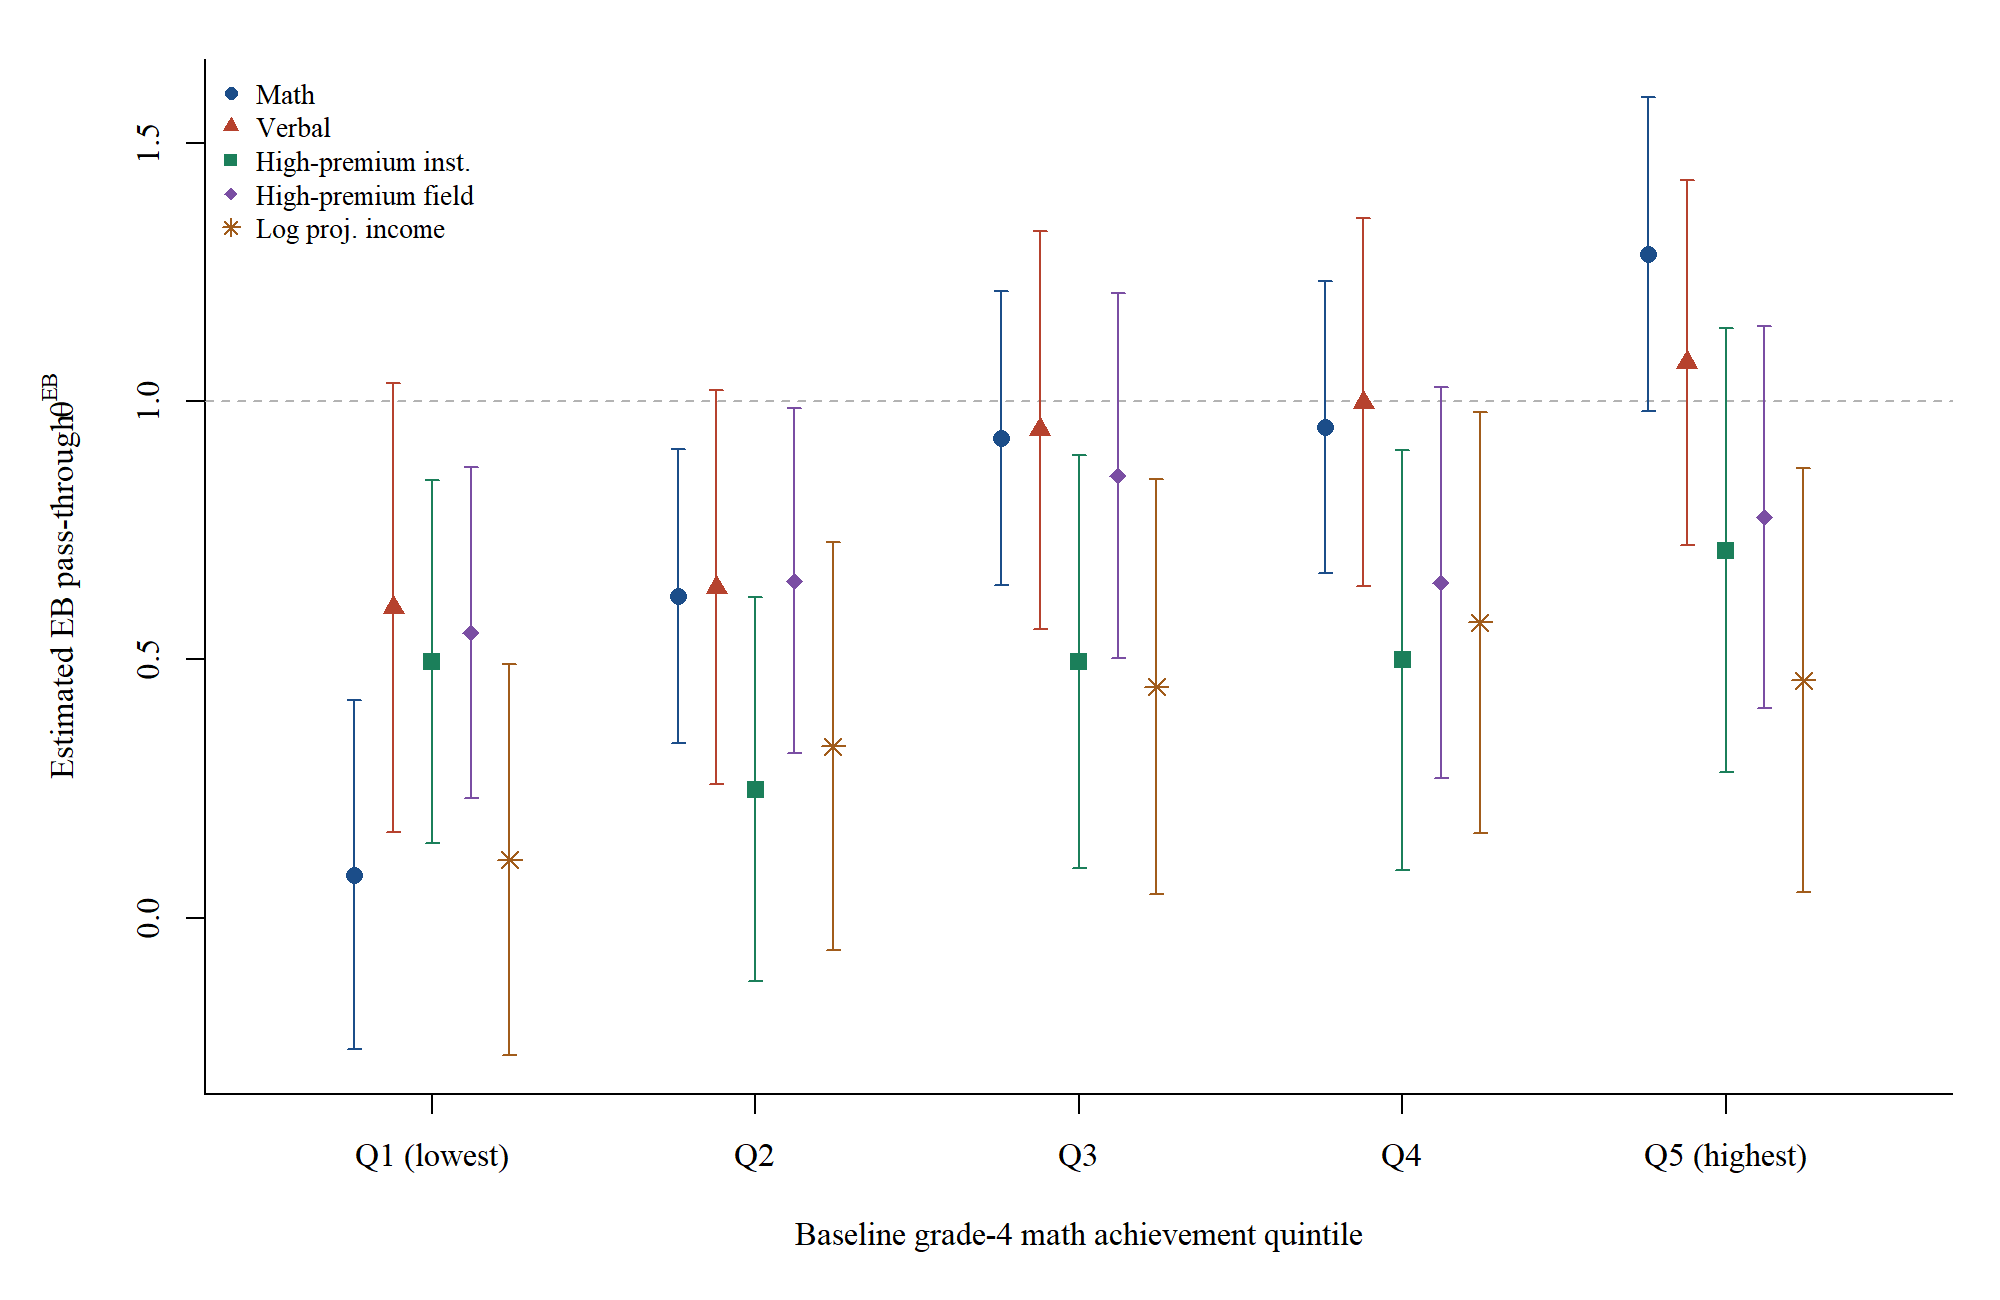
\includegraphics[width=.9\textwidth]{../../output/figures/results_section/simce4_math_quintile_primary_five_eb.png}
%\caption{EB scalar school-value IV estimates by baseline grade-4 math achievement quintile}
%\label{fig:simce4-math-quintile-primary-five-eb}
%\end{figure}
%\begin{table}[!htbp]
\centering
\caption{Differences in EB pass-through relative to the middle quintile}
\label{tab:simce4-math-quintile-primary-five-eb-contrasts-q3}
\small
\resizebox{\textwidth}{!}{%
\begin{tabular}{lccccc}
\toprule
 & \multicolumn{2}{c}{Exams} & \multicolumn{3}{c}{Higher ed. choices} \\
\cmidrule(lr){2-3} \cmidrule(lr){4-6}
Comparison & Math & Verbal & High-premium inst. & High-premium field & Log proj. income \\
\midrule
$Q1-Q3$ & -0.846*** & -0.345 & 0.001 & -0.304 & -0.335 \\
 & (0.225) & (0.296) & (0.272) & (0.243) & (0.282) \\
$Q2-Q3$ & -0.306 & -0.305 & -0.247 & -0.203 & -0.115 \\
 & (0.205) & (0.277) & (0.278) & (0.248) & (0.287) \\
$Q4-Q3$ & 0.022 & 0.053 & 0.003 & -0.207 & 0.125 \\
 & (0.205) & (0.268) & (0.291) & (0.264) & (0.292) \\
$Q5-Q3$ & 0.356* & 0.130 & 0.216 & -0.080 & 0.013 \\
 & (0.212) & (0.267) & (0.300) & (0.261) & (0.293) \\
\bottomrule
\end{tabular}
}
\par\medskip
\footnotesize
\begin{minipage}{\textwidth}
Notes: Each entry reports $\widehat{\theta}^{EB}_{Q_q} - \widehat{\theta}^{EB}_{Q3}$ for the indicated baseline grade-4 math achievement quintile. Heteroskedasticity-robust standard errors are reported in parentheses. Because quintile samples are disjoint, the contrast variance is the sum of the two coefficient variances. $^{*}p<0.10$, $^{**}p<0.05$, $^{***}p<0.01$.
\end{minipage}
\end{table}

%\FloatBarrier
%
%\subsection{Heterogeneity by Gender}
%
%I next ask whether the forecast estimates differ by gender.
%Gender is measured from the grade-8 enrollment records used to construct the linked student panel, so this split is predetermined relative to high-school assignment and does not rely on SAE or admission-test records.
%Figure~\ref{fig:primary-five-eb-by-gender} reports the five EB forecast estimates separately for boys and girls.
%Table~\ref{tab:primary-five-eb-gender-contrasts} reports the corresponding difference, girls relative to boys.
%
%The estimates are positive for both groups across all five outcomes.
%For achievement, however, the point estimates are larger for girls.
%The math pass-through estimate is 0.703 for boys and 1.053 for girls, a difference of 0.349 ($p=0.017$).
%The verbal estimate is 0.685 for boys and 1.066 for girls, a difference of 0.382 ($p=0.029$).
%Thus, lottery-induced movement toward schools with higher achievement value added appears to translate more strongly into measured achievement gains for girls.
%
%For higher-education choices, the gender differences are noticeably smaller.
%The point estimates for high-premium-institution enrollment and high-premium-field enrollment are also larger for girls, but neither difference is statistically significant.
%For log projected program income, the point estimate is slightly larger for boys, and the difference is close to zero.
%Overall, the gender split suggests meaningful heterogeneity in achievement pass-through, but does not provide evidence that the school effects on higher-education choices differ systematically between boys and girls.
%
%\begin{figure}[!htbp]
%\centering
%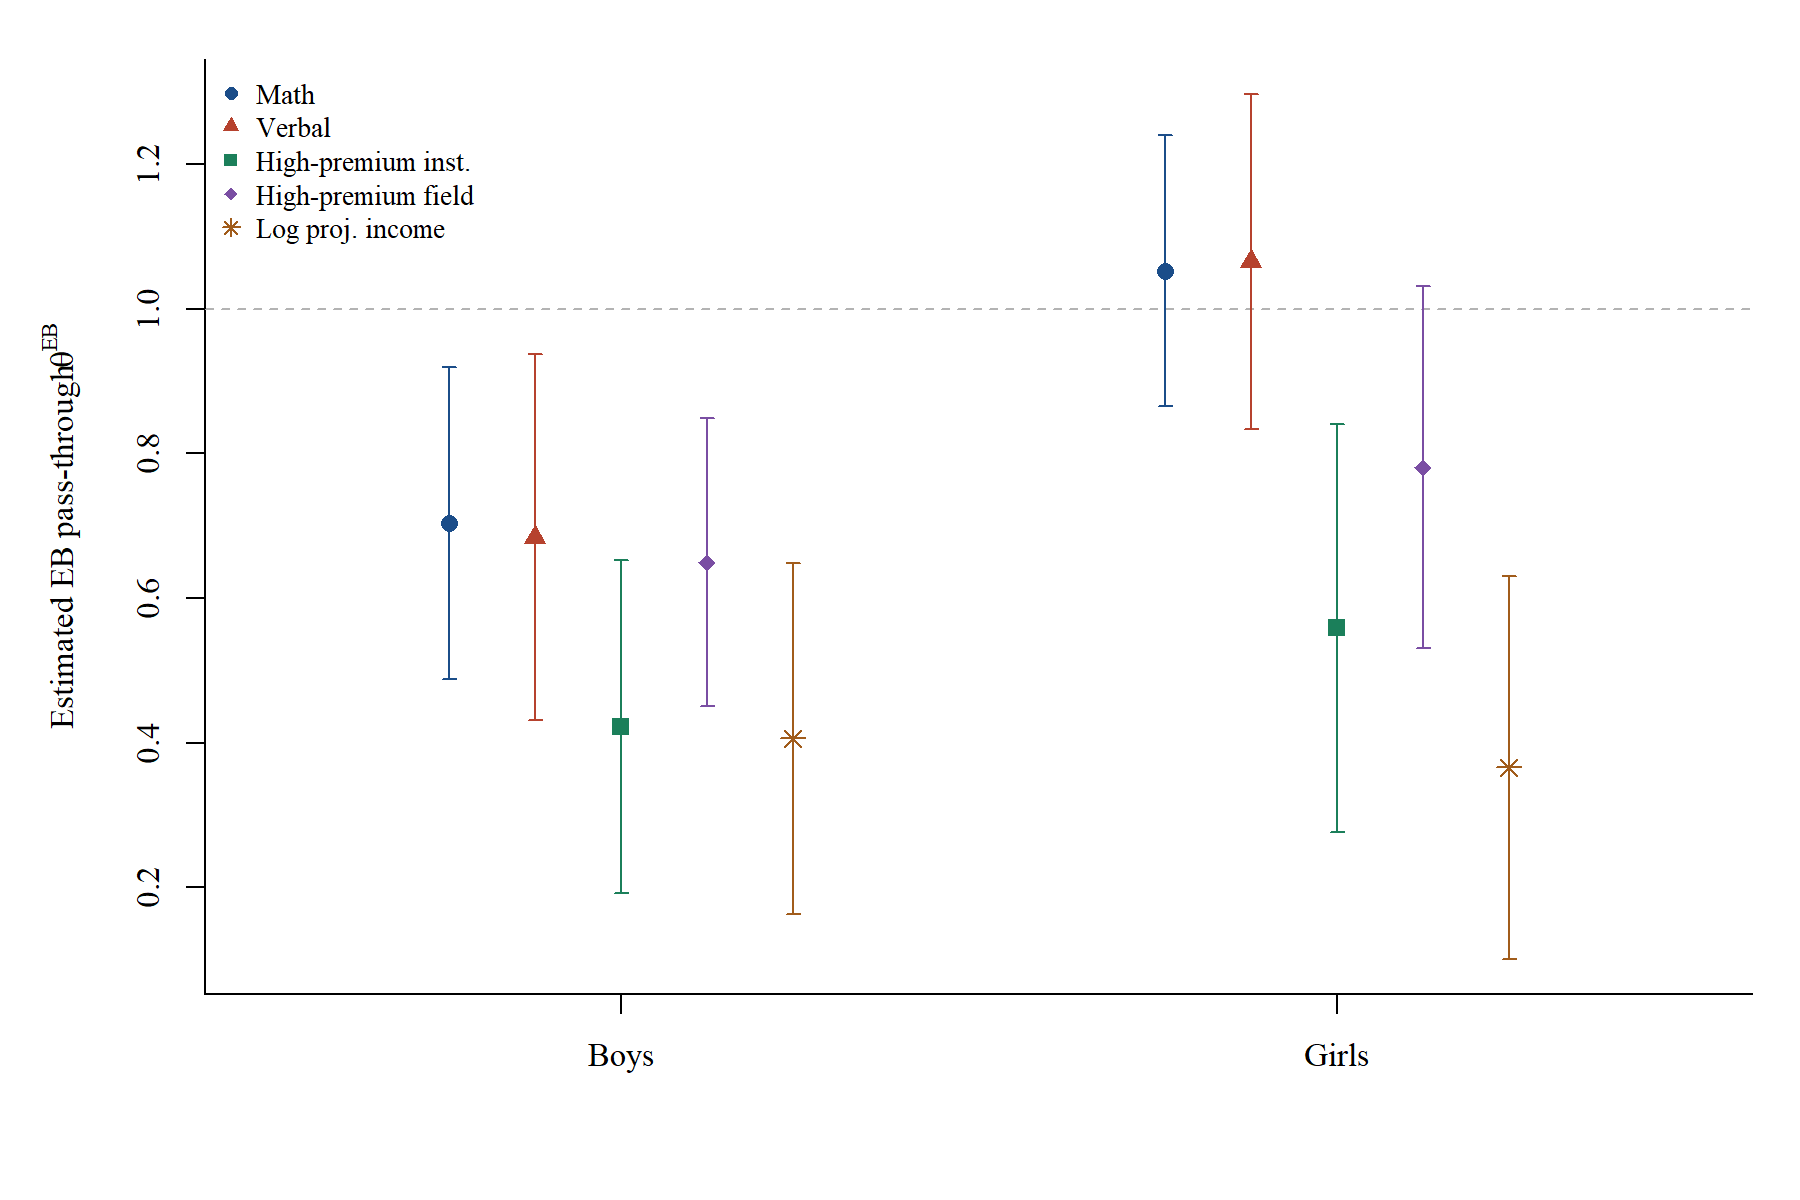
\includegraphics[width=.9\textwidth]{../../output/figures/results_section/primary_five_eb_by_gender.png}
%\caption{EB scalar school-value IV estimates by gender}
%\label{fig:primary-five-eb-by-gender}
%\end{figure}
%\begin{table}[!htbp]
\centering
\caption{Gender differences in EB pass-through}
\label{tab:primary-five-eb-gender-contrasts}
\small
\resizebox{\textwidth}{!}{%
\begin{tabular}{lccccc}
\toprule
 & \multicolumn{2}{c}{Exams} & \multicolumn{3}{c}{Higher ed. choices} \\
\cmidrule(lr){2-3} \cmidrule(lr){4-6}
Comparison & Math & Verbal & High-premium inst. & High-premium field & Log proj. income \\
\midrule
Girls $-$ Boys & 0.349** & 0.382** & 0.137 & 0.131 & -0.040 \\
 & (0.146) & (0.175) & (0.186) & (0.163) & (0.183) \\
\bottomrule
\end{tabular}
}
\par\medskip
\footnotesize
\begin{minipage}{\textwidth}
Notes: Each entry reports the difference in the EB pass-through estimate for girls relative to boys. Heteroskedasticity-robust standard errors are reported in parentheses. Because the two gender samples are disjoint, the contrast variance is the sum of the two coefficient variances. $^{*}p<0.10$, $^{**}p<0.05$, $^{***}p<0.01$.
\end{minipage}
\end{table}

%\FloatBarrier
%
%
%
%\subsection{Ordered Value-Added Horse Race for Projected Income}
%
%The scalar estimates above treat each outcome-specific value-added measure one at a time.
%I next ask whether the labor-market-relevant signal in projected program income is exhausted by math value added.
%This is a stricter question than asking whether schools affect projected income in the scalar specification.
%Schools that raise math achievement may also raise projected income, but high schools may affect later labor-market prospects through other margins: the institutions students attend and the fields they enter.
%The ordered horse race therefore tests which value-added dimensions retain predictive content for projected income as additional dimensions are added.
%
%Figure~\ref{fig:va-correlation-panels}, panel (a), first compares math and verbal value added as an achievement benchmark.
%The two achievement measures are strongly related across schools, with a correlation of 0.659.
%Panel (b) then compares math value added with high-premium-field value added.
%That relationship is positive but much weaker, with a correlation of 0.273.
%This pattern suggests that field-choice value added is related to, but not reducible to, achievement value added.
%The ordered exercise below asks whether these less achievement-like dimensions carry signal for projected income once math value added is given the first place in the ordering.
%
%\begin{figure}[!htbp]
%\centering
%\subbottom[Math and verbal value added\label{fig:math-verbal-va-correlation}]{%
%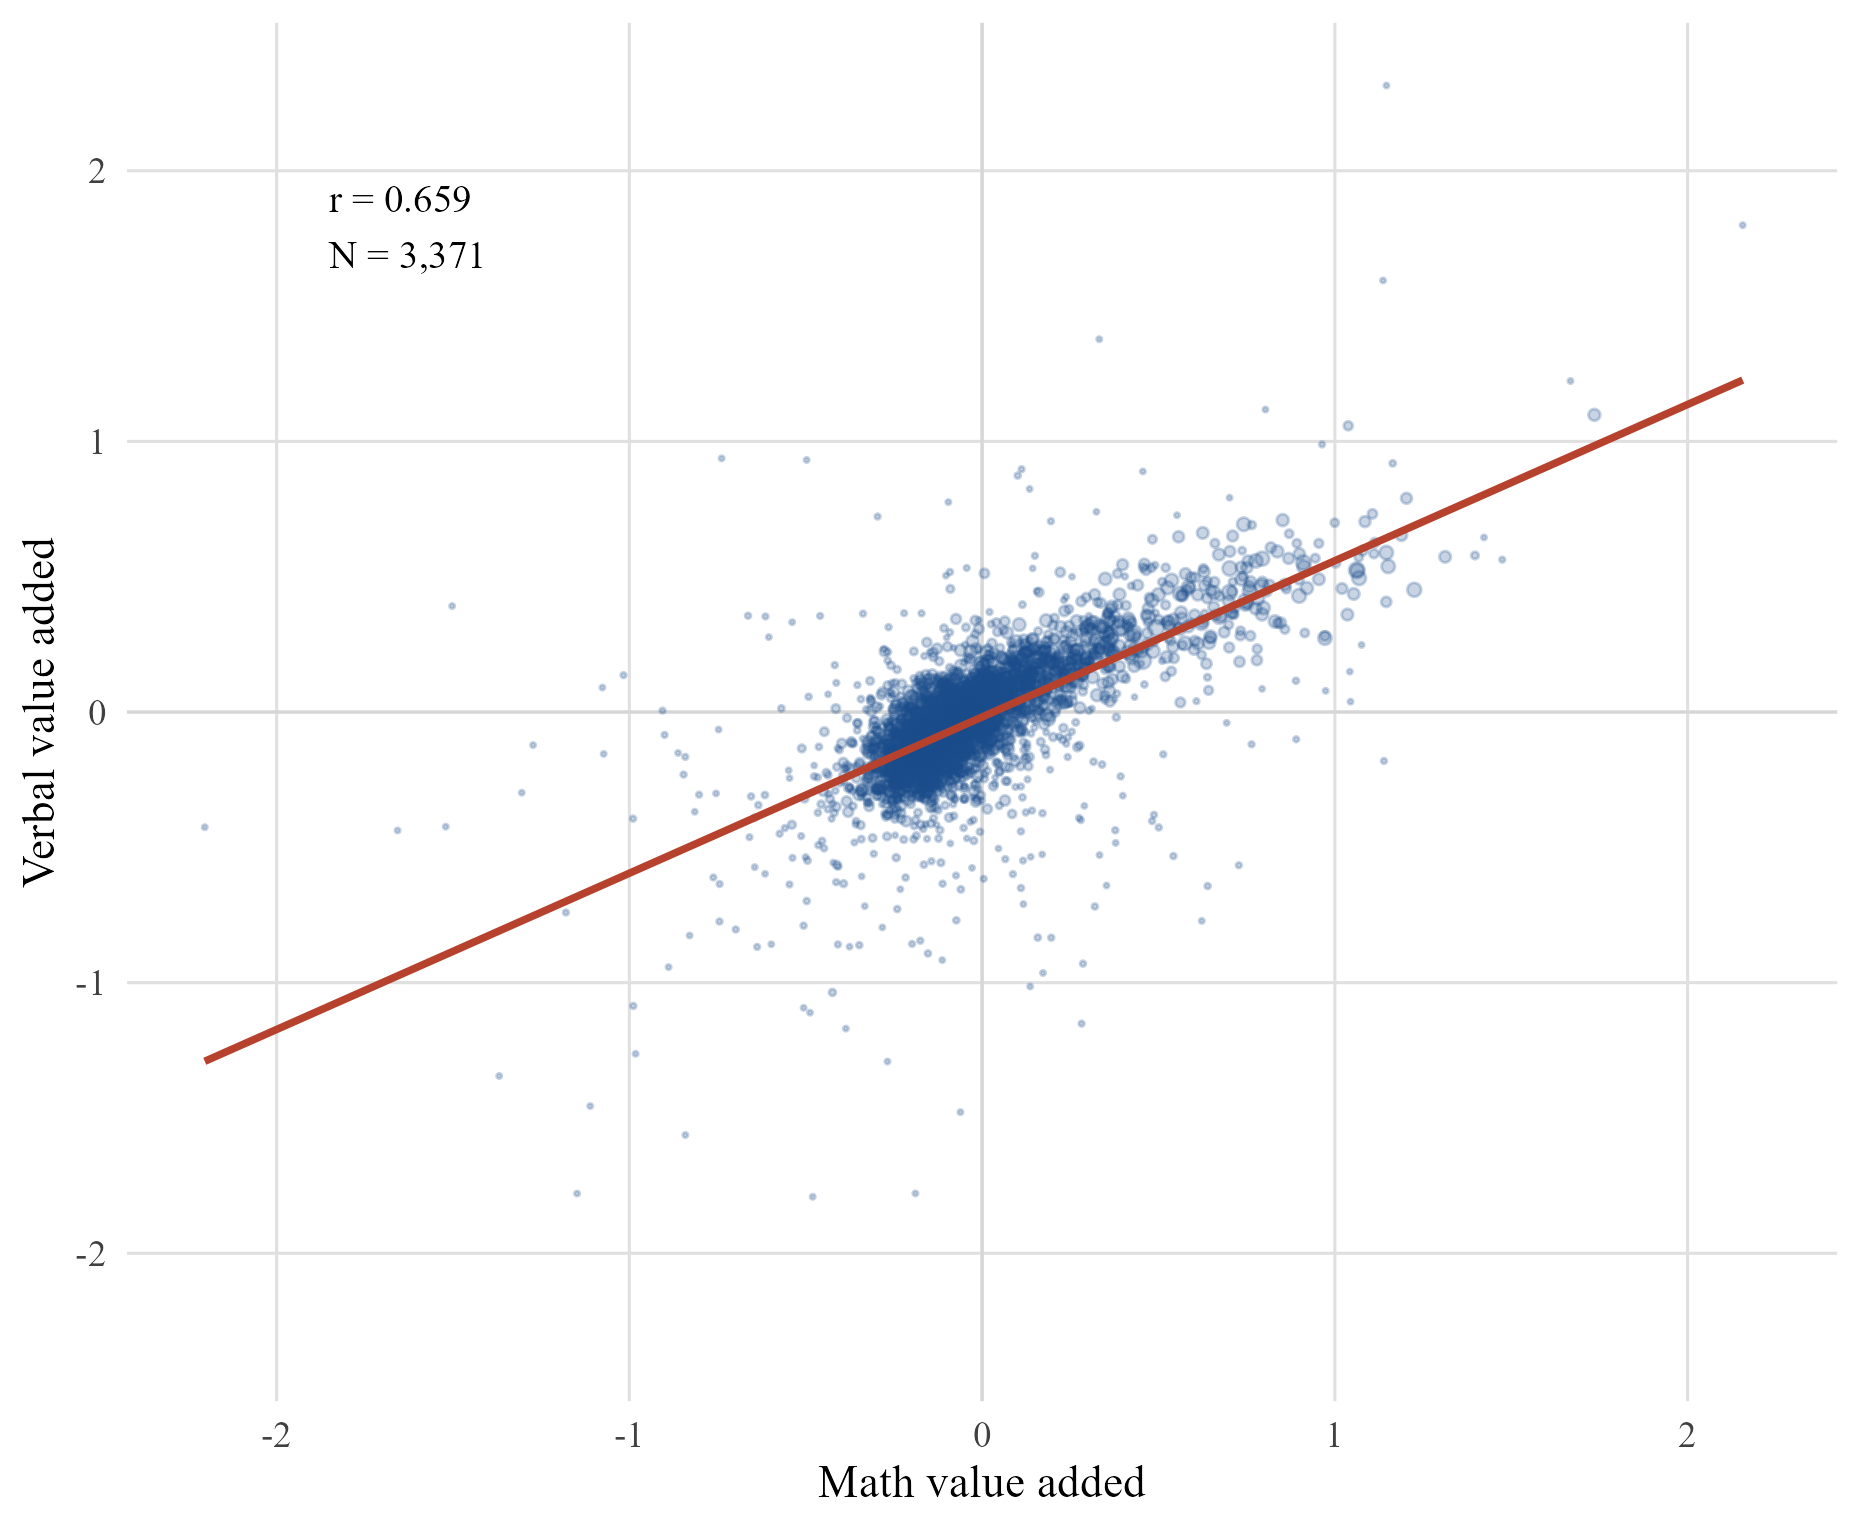
\includegraphics[width=.48\textwidth]{../../output/figures/results_section/math_language_va_correlation.png}%
%}
%\hfill
%\subbottom[Math and high-premium-field value added\label{fig:math-highpay-va-correlation}]{%
%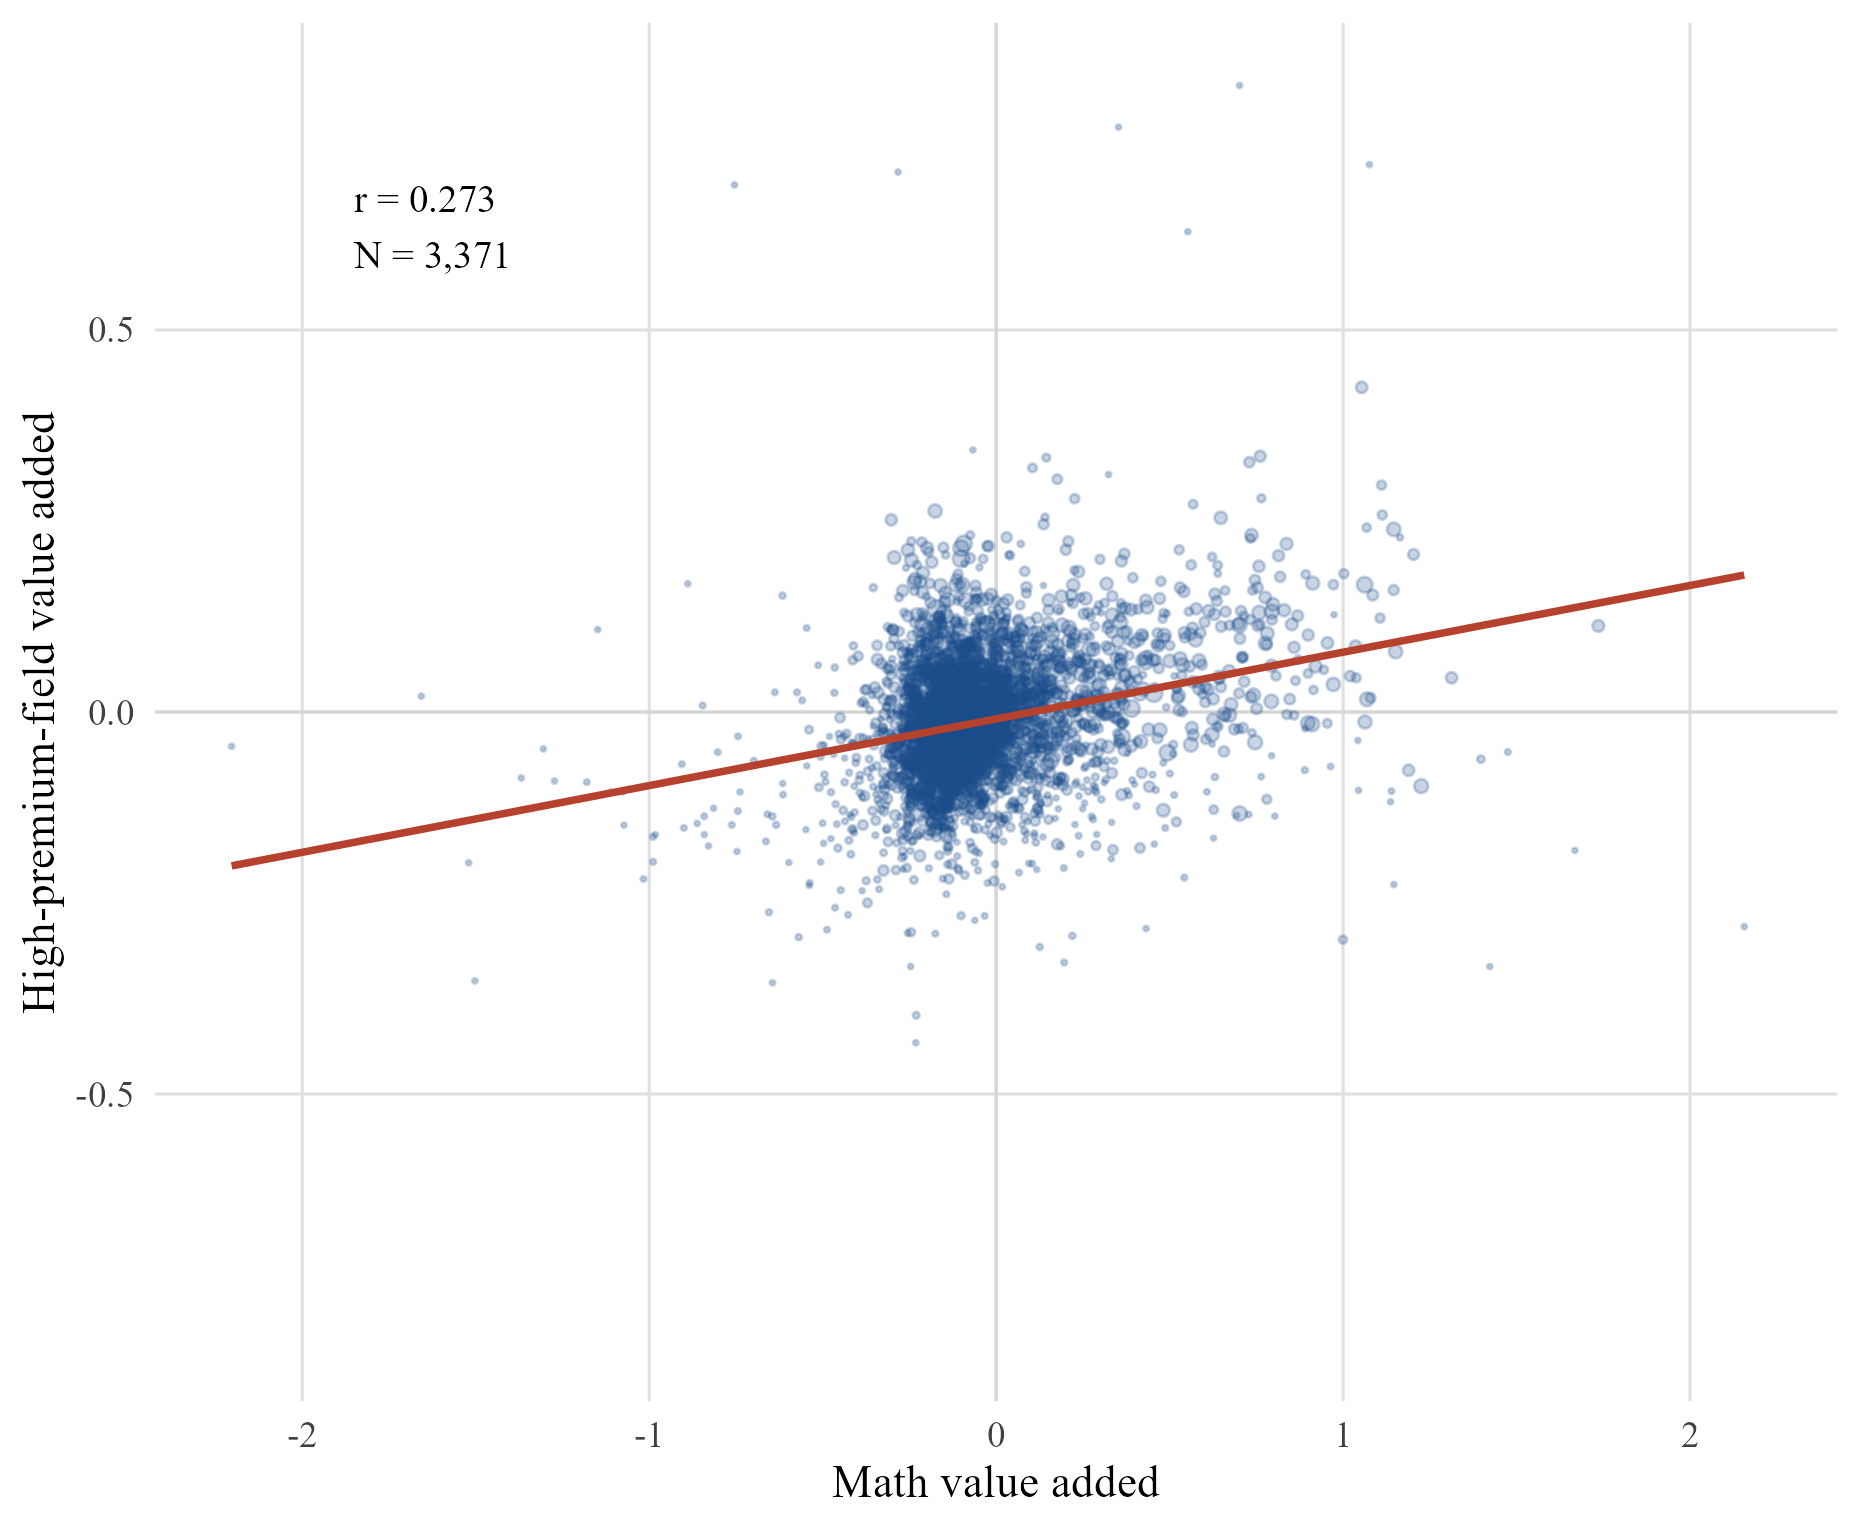
\includegraphics[width=.48\textwidth]{../../output/figures/results_section/math_highpay_va_correlation.png}%
%}
%\caption{Relationships between math, verbal, and high-premium-field observational value added}
%\label{fig:va-correlation-panels}
%\end{figure}
%\FloatBarrier
%
%I estimate a joint IV regression for log projected program income using the ordered EB value-added measures specified in equation~\ref{eq:ordered-va-iv}.
%Each attended school value is instrumented with the corresponding first-round offered-school value, and the regression controls for the assignment-risk expected value of each dimension.
%
%Table~\ref{tab:program-income-orthogonal-math-highinst-highpay} reports the estimates.
%Math value added has a small and statistically insignificant coefficient of $-0.056$.
%High-premium-institution value added net of math is positive, with an estimate of 0.286.
%High-premium-field value added net of math and high-premium-institution value added is positive and precisely estimated, with a coefficient of 0.366.
%These estimates are difficult to reconcile with a view in which math value added fully summarizes the school dimensions relevant for projected income.
%Instead, high schools appear to have labor-market-relevant value-added dimensions that are not captured by achievement value added alone.
%%The strongest evidence comes from the incremental high-premium-field dimension: schools that shift students toward high-premium fields also raise projected income after accounting for math and institution-choice value added.
%%The raw joint horse race gives the same qualitative message, but the ordered version makes the incremental interpretation more transparent.
%
%\begin{table}[!htbp]
\centering
\caption{Ordered IV horse race for log projected income}
\label{tab:program-income-orthogonal-math-highinst-highpay}
\begin{tabular}{lc}
\toprule
 & Log proj. income \\
\midrule
Math VA & -0.056 \\
 & (0.057) \\
High-premium-institution VA net of math & 0.286** \\
 & (0.143) \\
High-premium-field VA net of first two & 0.366*** \\
 & (0.096) \\
\midrule
N & 95,621 \\
\bottomrule
\end{tabular}
\par\medskip
\footnotesize
\begin{minipage}{\textwidth}
Notes: The dependent variable is log projected program income. The table reports an ordered horse-race IV. Math VA enters first; high-premium-institution VA is measured net of math VA; high-premium-field VA is measured net of the first two dimensions. This ordering is used to aid interpretation and does not make the coefficients structural returns to achievement, institutions, or fields. Attended-school values are instrumented with the corresponding first-round offered-school values, and the regression controls for the DA-probability expected value of each dimension, cohort, grade-4 SIMCE math and language, gender, and age. Heteroskedasticity-robust standard errors are reported in parentheses. $^{*}p<0.10$, $^{**}p<0.05$, $^{***}p<0.01$.
\end{minipage}
\end{table}

%
\FloatBarrier

\clearpage 
\section{Conclusion}

This paper asks whether high schools causally affect higher-education choices, and to what extent those effects are captured by observational value added.
I address this question by combining Chile's centralized school assignment system with linked administrative data.
I first estimate school value added for achievement and higher-education outcomes in a broad national panel, and then use lottery offers to ask whether schools that look better in observational value-added terms also produce larger causal effects.

% [FIX] Conclusion uses July numbers throughout.
The main estimates suggest meaningful pass-through.
The estimates are 0.884 for math, 0.885 for verbal achievement, 0.497 for high-premium-institution enrollment, 0.803 for high-premium-field enrollment, and 0.311 for log projected program income.
In practical terms, schools that observationally look better at raising achievement or higher-education outcomes also predict causal effects on those same outcomes, as I can confidently reject $\psi = 0$ in all dimensions of value added.
The results therefore show that the school assignment margin shifts later higher-education choices, not only test scores.

% [FIX] Heterogeneity results are commented out in the body.
The heterogeneity results show that the relationship is mostly stable across students, with noticeable exceptions.
Relative to students in the middle quintile of baseline math achievement, math value added is substantially less predictive in the bottom quintile and marginally more predictive in the top quintile.
At the same time, both verbal and math achievement show noticeable gender differences in their forecast coefficients.
These differences may suggest some caution when considering achievement value-added disclosure policies, especially in terms of their efficacy and equity across groups.
However, the non-achievement results are remarkably stable, making the common-effects approximation more plausible for those dimensions.

%For verbal achievement and the three higher-education outcomes, none of the differences relative to the middle quintile is statistically significant.
%These results point to meaningful heterogeneity in math pass-through, rather than a common pattern across outcomes or the baseline achievement distribution.

% [FIX] Horse race is commented out in the body. If it stays out, the var/cov results should carry this point instead.
Finally, I ask which dimensions of school value added predict gains in projected program income.
The ordered horse-race exercise enters math value added first, then high-premium-institution value added net of math, and finally high-premium-field value added net of the first two dimensions.
In this joint IV specification, math value added is small and statistically insignificant, while the two higher-education choice dimensions are positive and significant.
These results suggest that high schools differ along multiple dimensions in ways that are not captured by achievement alone.
In particular, schools affect higher-education decisions through dimensions not captured by math achievement, such as institution and field choice.
%The analysis does not determine whether these differences arise from counseling, information, expectations, peer norms, academic preparation, or other school practices.

These results show why achievement-based measures of school quality are incomplete.
As access to secondary and higher education expands, the consequences of schooling increasingly depend not only on learning and enrollment, but also on the decisions students make thereafter.
Accountability systems and school-choice policies centered on achievement may therefore overlook school effects that matter for the allocation of skills across fields, occupations, and sectors.

The results also qualify how higher-education choices should be interpreted.
Decisions not to continue to higher education, to avoid particular fields, or to attend lower-quality institutions are often interpreted as revealing stable preferences or privately optimal responses to expected returns.
Yet both expected returns and the options students perceive can be shaped by the information, expectations, academic preparation, and support they receive in high school.
A decision may therefore be privately optimal given beliefs and preparation that the high school helped produce, while still being causally affected by the school attended.
This possibility is especially important in settings where families have limited information about educational options and where access to counseling and other supports varies across schools.

%Future work should attempt to identify the specific channels that generate these effects and examine whether families value and respond to nontraditional measures of school value added.
%It should also study whether providing information on multiple dimensions of school quality changes school demand and later educational choices, and estimate the aggregate consequences of systematically ignoring these dimensions when students and funds are allocated across schools.




\clearpage
\printbibliography


\section{Appendix}

\input{../../output/tables/balance_table/balance_table_school_sector.tex}

\begin{table}[!htbp]
\centering
\caption{Eventual school by SAE application rank and first-round offer status: VA 2017--2020; SAE 2018--2020}
\label{tab:application-rank-takeup-maximum-data}
\begin{tabular}{lrrrrr}
\toprule
 & \multicolumn{2}{c}{Recorded first-round offer} & \multicolumn{2}{c}{No recorded first-round offer} & Difference \\
\cmidrule(lr){2-3} \cmidrule(lr){4-5}
Application position & N & Share & N & Share & First-round offer $-$ no offer \\
\midrule
Choice 1 & 141,462 & 39.1\% & 22,154 & 19.9\% & +19.2 pp \\
Choice 2 & 140,777 & 20.5\% & 21,929 & 8.7\% & +11.8 pp \\
Choice 3 & 117,346 & 12.7\% & 17,074 & 6.5\% & +6.1 pp \\
Any of top 3 & 141,462 & 69.5\% & 22,154 & 33.6\% & +35.8 pp \\
\bottomrule
\end{tabular}
\par\medskip
\footnotesize
\begin{minipage}{0.95\textwidth}
Notes: Each row reports the share whose most-time high school after grade 8 equals the indicated position in the student's SAE application list. Rank-specific denominators include students who submitted a school at that rank. The top-three denominator includes students with a first choice and counts attendance at any available choice among positions 1--3. Recorded first-round offer means a positive school identifier in the regular first-round SAE assignment record; it does not include later or supplementary assignment rounds.
\end{minipage}
\end{table}





\end{document}
